\documentclass[   ]{article}

% --- Estilo ICLR y paquetes requeridos ---
\usepackage{iclr2027_conference,times}

\iclrfinalcopy

% Comandos matemáticos y notación por defecto
%%%%% NEW MATH DEFINITIONS %%%%%

\usepackage{amsmath,amsfonts,bm}

% Mark sections of captions for referring to divisions of figures
\newcommand{\figleft}{{\em (Left)}}
\newcommand{\figcenter}{{\em (Center)}}
\newcommand{\figright}{{\em (Right)}}
\newcommand{\figtop}{{\em (Top)}}
\newcommand{\figbottom}{{\em (Bottom)}}
\newcommand{\captiona}{{\em (a)}}
\newcommand{\captionb}{{\em (b)}}
\newcommand{\captionc}{{\em (c)}}
\newcommand{\captiond}{{\em (d)}}

% Highlight a newly defined term
\newcommand{\newterm}[1]{{\bf #1}}


% Figure reference, lower-case.
\def\figref#1{figure~\ref{#1}}
% Figure reference, capital. For start of sentence
\def\Figref#1{Figure~\ref{#1}}
\def\twofigref#1#2{figures \ref{#1} and \ref{#2}}
\def\quadfigref#1#2#3#4{figures \ref{#1}, \ref{#2}, \ref{#3} and \ref{#4}}
% Section reference, lower-case.
\def\secref#1{section~\ref{#1}}
% Section reference, capital.
\def\Secref#1{Section~\ref{#1}}
% Reference to two sections.
\def\twosecrefs#1#2{sections \ref{#1} and \ref{#2}}
% Reference to three sections.
\def\secrefs#1#2#3{sections \ref{#1}, \ref{#2} and \ref{#3}}
% Reference to an equation, lower-case.
\def\eqref#1{equation~\ref{#1}}
% Reference to an equation, upper case
\def\Eqref#1{Equation~\ref{#1}}
% A raw reference to an equation---avoid using if possible
\def\plaineqref#1{\ref{#1}}
% Reference to a chapter, lower-case.
\def\chapref#1{chapter~\ref{#1}}
% Reference to an equation, upper case.
\def\Chapref#1{Chapter~\ref{#1}}
% Reference to a range of chapters
\def\rangechapref#1#2{chapters\ref{#1}--\ref{#2}}
% Reference to an algorithm, lower-case.
\def\algref#1{algorithm~\ref{#1}}
% Reference to an algorithm, upper case.
\def\Algref#1{Algorithm~\ref{#1}}
\def\twoalgref#1#2{algorithms \ref{#1} and \ref{#2}}
\def\Twoalgref#1#2{Algorithms \ref{#1} and \ref{#2}}
% Reference to a part, lower case
\def\partref#1{part~\ref{#1}}
% Reference to a part, upper case
\def\Partref#1{Part~\ref{#1}}
\def\twopartref#1#2{parts \ref{#1} and \ref{#2}}

\def\ceil#1{\lceil #1 \rceil}
\def\floor#1{\lfloor #1 \rfloor}
\def\1{\bm{1}}
\newcommand{\train}{\mathcal{D}}
\newcommand{\valid}{\mathcal{D_{\mathrm{valid}}}}
\newcommand{\test}{\mathcal{D_{\mathrm{test}}}}

\def\eps{{\epsilon}}


% Random variables
\def\reta{{\textnormal{$\eta$}}}
\def\ra{{\textnormal{a}}}
\def\rb{{\textnormal{b}}}
\def\rc{{\textnormal{c}}}
\def\rd{{\textnormal{d}}}
\def\re{{\textnormal{e}}}
\def\rf{{\textnormal{f}}}
\def\rg{{\textnormal{g}}}
\def\rh{{\textnormal{h}}}
\def\ri{{\textnormal{i}}}
\def\rj{{\textnormal{j}}}
\def\rk{{\textnormal{k}}}
\def\rl{{\textnormal{l}}}
% rm is already a command, just don't name any random variables m
\def\rn{{\textnormal{n}}}
\def\ro{{\textnormal{o}}}
\def\rp{{\textnormal{p}}}
\def\rq{{\textnormal{q}}}
\def\rr{{\textnormal{r}}}
\def\rs{{\textnormal{s}}}
\def\rt{{\textnormal{t}}}
\def\ru{{\textnormal{u}}}
\def\rv{{\textnormal{v}}}
\def\rw{{\textnormal{w}}}
\def\rx{{\textnormal{x}}}
\def\ry{{\textnormal{y}}}
\def\rz{{\textnormal{z}}}

% Random vectors
\def\rvepsilon{{\mathbf{\epsilon}}}
\def\rvtheta{{\mathbf{\theta}}}
\def\rva{{\mathbf{a}}}
\def\rvb{{\mathbf{b}}}
\def\rvc{{\mathbf{c}}}
\def\rvd{{\mathbf{d}}}
\def\rve{{\mathbf{e}}}
\def\rvf{{\mathbf{f}}}
\def\rvg{{\mathbf{g}}}
\def\rvh{{\mathbf{h}}}
\def\rvu{{\mathbf{i}}}
\def\rvj{{\mathbf{j}}}
\def\rvk{{\mathbf{k}}}
\def\rvl{{\mathbf{l}}}
\def\rvm{{\mathbf{m}}}
\def\rvn{{\mathbf{n}}}
\def\rvo{{\mathbf{o}}}
\def\rvp{{\mathbf{p}}}
\def\rvq{{\mathbf{q}}}
\def\rvr{{\mathbf{r}}}
\def\rvs{{\mathbf{s}}}
\def\rvt{{\mathbf{t}}}
\def\rvu{{\mathbf{u}}}
\def\rvv{{\mathbf{v}}}
\def\rvw{{\mathbf{w}}}
\def\rvx{{\mathbf{x}}}
\def\rvy{{\mathbf{y}}}
\def\rvz{{\mathbf{z}}}

% Elements of random vectors
\def\erva{{\textnormal{a}}}
\def\ervb{{\textnormal{b}}}
\def\ervc{{\textnormal{c}}}
\def\ervd{{\textnormal{d}}}
\def\erve{{\textnormal{e}}}
\def\ervf{{\textnormal{f}}}
\def\ervg{{\textnormal{g}}}
\def\ervh{{\textnormal{h}}}
\def\ervi{{\textnormal{i}}}
\def\ervj{{\textnormal{j}}}
\def\ervk{{\textnormal{k}}}
\def\ervl{{\textnormal{l}}}
\def\ervm{{\textnormal{m}}}
\def\ervn{{\textnormal{n}}}
\def\ervo{{\textnormal{o}}}
\def\ervp{{\textnormal{p}}}
\def\ervq{{\textnormal{q}}}
\def\ervr{{\textnormal{r}}}
\def\ervs{{\textnormal{s}}}
\def\ervt{{\textnormal{t}}}
\def\ervu{{\textnormal{u}}}
\def\ervv{{\textnormal{v}}}
\def\ervw{{\textnormal{w}}}
\def\ervx{{\textnormal{x}}}
\def\ervy{{\textnormal{y}}}
\def\ervz{{\textnormal{z}}}

% Random matrices
\def\rmA{{\mathbf{A}}}
\def\rmB{{\mathbf{B}}}
\def\rmC{{\mathbf{C}}}
\def\rmD{{\mathbf{D}}}
\def\rmE{{\mathbf{E}}}
\def\rmF{{\mathbf{F}}}
\def\rmG{{\mathbf{G}}}
\def\rmH{{\mathbf{H}}}
\def\rmI{{\mathbf{I}}}
\def\rmJ{{\mathbf{J}}}
\def\rmK{{\mathbf{K}}}
\def\rmL{{\mathbf{L}}}
\def\rmM{{\mathbf{M}}}
\def\rmN{{\mathbf{N}}}
\def\rmO{{\mathbf{O}}}
\def\rmP{{\mathbf{P}}}
\def\rmQ{{\mathbf{Q}}}
\def\rmR{{\mathbf{R}}}
\def\rmS{{\mathbf{S}}}
\def\rmT{{\mathbf{T}}}
\def\rmU{{\mathbf{U}}}
\def\rmV{{\mathbf{V}}}
\def\rmW{{\mathbf{W}}}
\def\rmX{{\mathbf{X}}}
\def\rmY{{\mathbf{Y}}}
\def\rmZ{{\mathbf{Z}}}

% Elements of random matrices
\def\ermA{{\textnormal{A}}}
\def\ermB{{\textnormal{B}}}
\def\ermC{{\textnormal{C}}}
\def\ermD{{\textnormal{D}}}
\def\ermE{{\textnormal{E}}}
\def\ermF{{\textnormal{F}}}
\def\ermG{{\textnormal{G}}}
\def\ermH{{\textnormal{H}}}
\def\ermI{{\textnormal{I}}}
\def\ermJ{{\textnormal{J}}}
\def\ermK{{\textnormal{K}}}
\def\ermL{{\textnormal{L}}}
\def\ermM{{\textnormal{M}}}
\def\ermN{{\textnormal{N}}}
\def\ermO{{\textnormal{O}}}
\def\ermP{{\textnormal{P}}}
\def\ermQ{{\textnormal{Q}}}
\def\ermR{{\textnormal{R}}}
\def\ermS{{\textnormal{S}}}
\def\ermT{{\textnormal{T}}}
\def\ermU{{\textnormal{U}}}
\def\ermV{{\textnormal{V}}}
\def\ermW{{\textnormal{W}}}
\def\ermX{{\textnormal{X}}}
\def\ermY{{\textnormal{Y}}}
\def\ermZ{{\textnormal{Z}}}

% Vectors
\def\vzero{{\bm{0}}}
\def\vone{{\bm{1}}}
\def\vmu{{\bm{\mu}}}
\def\vtheta{{\bm{\theta}}}
\def\va{{\bm{a}}}
\def\vb{{\bm{b}}}
\def\vc{{\bm{c}}}
\def\vd{{\bm{d}}}
\def\ve{{\bm{e}}}
\def\vf{{\bm{f}}}
\def\vg{{\bm{g}}}
\def\vh{{\bm{h}}}
\def\vi{{\bm{i}}}
\def\vj{{\bm{j}}}
\def\vk{{\bm{k}}}
\def\vl{{\bm{l}}}
\def\vm{{\bm{m}}}
\def\vn{{\bm{n}}}
\def\vo{{\bm{o}}}
\def\vp{{\bm{p}}}
\def\vq{{\bm{q}}}
\def\vr{{\bm{r}}}
\def\vs{{\bm{s}}}
\def\vt{{\bm{t}}}
\def\vu{{\bm{u}}}
\def\vv{{\bm{v}}}
\def\vw{{\bm{w}}}
\def\vx{{\bm{x}}}
\def\vy{{\bm{y}}}
\def\vz{{\bm{z}}}

% Elements of vectors
\def\evalpha{{\alpha}}
\def\evbeta{{\beta}}
\def\evepsilon{{\epsilon}}
\def\evlambda{{\lambda}}
\def\evomega{{\omega}}
\def\evmu{{\mu}}
\def\evpsi{{\psi}}
\def\evsigma{{\sigma}}
\def\evtheta{{\theta}}
\def\eva{{a}}
\def\evb{{b}}
\def\evc{{c}}
\def\evd{{d}}
\def\eve{{e}}
\def\evf{{f}}
\def\evg{{g}}
\def\evh{{h}}
\def\evi{{i}}
\def\evj{{j}}
\def\evk{{k}}
\def\evl{{l}}
\def\evm{{m}}
\def\evn{{n}}
\def\evo{{o}}
\def\evp{{p}}
\def\evq{{q}}
\def\evr{{r}}
\def\evs{{s}}
\def\evt{{t}}
\def\evu{{u}}
\def\evv{{v}}
\def\evw{{w}}
\def\evx{{x}}
\def\evy{{y}}
\def\evz{{z}}

% Matrix
\def\mA{{\bm{A}}}
\def\mB{{\bm{B}}}
\def\mC{{\bm{C}}}
\def\mD{{\bm{D}}}
\def\mE{{\bm{E}}}
\def\mF{{\bm{F}}}
\def\mG{{\bm{G}}}
\def\mH{{\bm{H}}}
\def\mI{{\bm{I}}}
\def\mJ{{\bm{J}}}
\def\mK{{\bm{K}}}
\def\mL{{\bm{L}}}
\def\mM{{\bm{M}}}
\def\mN{{\bm{N}}}
\def\mO{{\bm{O}}}
\def\mP{{\bm{P}}}
\def\mQ{{\bm{Q}}}
\def\mR{{\bm{R}}}
\def\mS{{\bm{S}}}
\def\mT{{\bm{T}}}
\def\mU{{\bm{U}}}
\def\mV{{\bm{V}}}
\def\mW{{\bm{W}}}
\def\mX{{\bm{X}}}
\def\mY{{\bm{Y}}}
\def\mZ{{\bm{Z}}}
\def\mBeta{{\bm{\beta}}}
\def\mPhi{{\bm{\Phi}}}
\def\mLambda{{\bm{\Lambda}}}
\def\mSigma{{\bm{\Sigma}}}

% Tensor
\DeclareMathAlphabet{\mathsfit}{\encodingdefault}{\sfdefault}{m}{sl}
\SetMathAlphabet{\mathsfit}{bold}{\encodingdefault}{\sfdefault}{bx}{n}
\newcommand{\tens}[1]{\bm{\mathsfit{#1}}}
\def\tA{{\tens{A}}}
\def\tB{{\tens{B}}}
\def\tC{{\tens{C}}}
\def\tD{{\tens{D}}}
\def\tE{{\tens{E}}}
\def\tF{{\tens{F}}}
\def\tG{{\tens{G}}}
\def\tH{{\tens{H}}}
\def\tI{{\tens{I}}}
\def\tJ{{\tens{J}}}
\def\tK{{\tens{K}}}
\def\tL{{\tens{L}}}
\def\tM{{\tens{M}}}
\def\tN{{\tens{N}}}
\def\tO{{\tens{O}}}
\def\tP{{\tens{P}}}
\def\tQ{{\tens{Q}}}
\def\tR{{\tens{R}}}
\def\tS{{\tens{S}}}
\def\tT{{\tens{T}}}
\def\tU{{\tens{U}}}
\def\tV{{\tens{V}}}
\def\tW{{\tens{W}}}
\def\tX{{\tens{X}}}
\def\tY{{\tens{Y}}}
\def\tZ{{\tens{Z}}}


% Graph
\def\gA{{\mathcal{A}}}
\def\gB{{\mathcal{B}}}
\def\gC{{\mathcal{C}}}
\def\gD{{\mathcal{D}}}
\def\gE{{\mathcal{E}}}
\def\gF{{\mathcal{F}}}
\def\gG{{\mathcal{G}}}
\def\gH{{\mathcal{H}}}
\def\gI{{\mathcal{I}}}
\def\gJ{{\mathcal{J}}}
\def\gK{{\mathcal{K}}}
\def\gL{{\mathcal{L}}}
\def\gM{{\mathcal{M}}}
\def\gN{{\mathcal{N}}}
\def\gO{{\mathcal{O}}}
\def\gP{{\mathcal{P}}}
\def\gQ{{\mathcal{Q}}}
\def\gR{{\mathcal{R}}}
\def\gS{{\mathcal{S}}}
\def\gT{{\mathcal{T}}}
\def\gU{{\mathcal{U}}}
\def\gV{{\mathcal{V}}}
\def\gW{{\mathcal{W}}}
\def\gX{{\mathcal{X}}}
\def\gY{{\mathcal{Y}}}
\def\gZ{{\mathcal{Z}}}

% Sets
\def\sA{{\mathbb{A}}}
\def\sB{{\mathbb{B}}}
\def\sC{{\mathbb{C}}}
\def\sD{{\mathbb{D}}}
% Don't use a set called E, because this would be the same as our symbol
% for expectation.
\def\sF{{\mathbb{F}}}
\def\sG{{\mathbb{G}}}
\def\sH{{\mathbb{H}}}
\def\sI{{\mathbb{I}}}
\def\sJ{{\mathbb{J}}}
\def\sK{{\mathbb{K}}}
\def\sL{{\mathbb{L}}}
\def\sM{{\mathbb{M}}}
\def\sN{{\mathbb{N}}}
\def\sO{{\mathbb{O}}}
\def\sP{{\mathbb{P}}}
\def\sQ{{\mathbb{Q}}}
\def\sR{{\mathbb{R}}}
\def\sS{{\mathbb{S}}}
\def\sT{{\mathbb{T}}}
\def\sU{{\mathbb{U}}}
\def\sV{{\mathbb{V}}}
\def\sW{{\mathbb{W}}}
\def\sX{{\mathbb{X}}}
\def\sY{{\mathbb{Y}}}
\def\sZ{{\mathbb{Z}}}

% Entries of a matrix
\def\emLambda{{\Lambda}}
\def\emA{{A}}
\def\emB{{B}}
\def\emC{{C}}
\def\emD{{D}}
\def\emE{{E}}
\def\emF{{F}}
\def\emG{{G}}
\def\emH{{H}}
\def\emI{{I}}
\def\emJ{{J}}
\def\emK{{K}}
\def\emL{{L}}
\def\emM{{M}}
\def\emN{{N}}
\def\emO{{O}}
\def\emP{{P}}
\def\emQ{{Q}}
\def\emR{{R}}
\def\emS{{S}}
\def\emT{{T}}
\def\emU{{U}}
\def\emV{{V}}
\def\emW{{W}}
\def\emX{{X}}
\def\emY{{Y}}
\def\emZ{{Z}}
\def\emSigma{{\Sigma}}

% entries of a tensor
% Same font as tensor, without \bm wrapper
\newcommand{\etens}[1]{\mathsfit{#1}}
\def\etLambda{{\etens{\Lambda}}}
\def\etA{{\etens{A}}}
\def\etB{{\etens{B}}}
\def\etC{{\etens{C}}}
\def\etD{{\etens{D}}}
\def\etE{{\etens{E}}}
\def\etF{{\etens{F}}}
\def\etG{{\etens{G}}}
\def\etH{{\etens{H}}}
\def\etI{{\etens{I}}}
\def\etJ{{\etens{J}}}
\def\etK{{\etens{K}}}
\def\etL{{\etens{L}}}
\def\etM{{\etens{M}}}
\def\etN{{\etens{N}}}
\def\etO{{\etens{O}}}
\def\etP{{\etens{P}}}
\def\etQ{{\etens{Q}}}
\def\etR{{\etens{R}}}
\def\etS{{\etens{S}}}
\def\etT{{\etens{T}}}
\def\etU{{\etens{U}}}
\def\etV{{\etens{V}}}
\def\etW{{\etens{W}}}
\def\etX{{\etens{X}}}
\def\etY{{\etens{Y}}}
\def\etZ{{\etens{Z}}}

% The true underlying data generating distribution
\newcommand{\pdata}{p_{\rm{data}}}
% The empirical distribution defined by the training set
\newcommand{\ptrain}{\hat{p}_{\rm{data}}}
\newcommand{\Ptrain}{\hat{P}_{\rm{data}}}
% The model distribution
\newcommand{\pmodel}{p_{\rm{model}}}
\newcommand{\Pmodel}{P_{\rm{model}}}
\newcommand{\ptildemodel}{\tilde{p}_{\rm{model}}}
% Stochastic autoencoder distributions
\newcommand{\pencode}{p_{\rm{encoder}}}
\newcommand{\pdecode}{p_{\rm{decoder}}}
\newcommand{\precons}{p_{\rm{reconstruct}}}

\newcommand{\laplace}{\mathrm{Laplace}} % Laplace distribution

\newcommand{\E}{\mathbb{E}}
\newcommand{\Ls}{\mathcal{L}}
\newcommand{\R}{\mathbb{R}}
\newcommand{\emp}{\tilde{p}}
\newcommand{\lr}{\alpha}
\newcommand{\reg}{\lambda}
\newcommand{\rect}{\mathrm{rectifier}}
\newcommand{\softmax}{\mathrm{softmax}}
\newcommand{\sigmoid}{\sigma}
\newcommand{\softplus}{\zeta}
\newcommand{\KL}{D_{\mathrm{KL}}}
\newcommand{\Var}{\mathrm{Var}}
\newcommand{\standarderror}{\mathrm{SE}}
\newcommand{\Cov}{\mathrm{Cov}}
% Wolfram Mathworld says $L^2$ is for function spaces and $\ell^2$ is for vectors
% But then they seem to use $L^2$ for vectors throughout the site, and so does
% wikipedia.
\newcommand{\normlzero}{L^0}
\newcommand{\normlone}{L^1}
\newcommand{\normltwo}{L^2}
\newcommand{\normlp}{L^p}
\newcommand{\normmax}{L^\infty}

\newcommand{\parents}{Pa} % See usage in notation.tex. Chosen to match Daphne's book.

\DeclareMathOperator*{\argmax}{arg\,max}
\DeclareMathOperator*{\argmin}{arg\,min}

\DeclareMathOperator{\sign}{sign}
\DeclareMathOperator{\Tr}{Tr}
\let\ab\allowbreak


\usepackage{url}
\usepackage{graphicx}
\usepackage{booktabs}
\usepackage{amsmath,amssymb,amsfonts}
\usepackage{longtable}
\usepackage{ltablex}
\usepackage{array}
\usepackage{calc}
\usepackage{enumitem}
\usepackage{microtype}
\usepackage{tabularx}
\usepackage{xltabular}
\usepackage{inconsolata}
\usepackage[T1]{fontenc}
\usepackage{seqsplit}
\usepackage{float}
\usepackage{graphicx}
\graphicspath{{./images}}
\usepackage{hyperref}
\usepackage{caption}
\usepackage{soul}
\usepackage[table]{xcolor}
\usepackage{enumitem}
\usepackage{adjustbox}

\let\oldtexttt\texttt
\renewcommand{\texttt}[1]{\oldtexttt{\itshape #1}}

% Compatibilidad para títulos y secciones de Pandoc
\providecommand{\hypertarget}[2]{#2}

% Definición requerida por Pandoc para las listas
\providecommand{\tightlist}{%
	\setlength{\itemsep}{0pt}\setlength{\parskip}{0pt}}

\makeatletter
\@ifundefined{c@none}{\newcounter{none}}{}
\makeatother

% --- Metadatos del Título y Autores ---
\title{Canonicalization for DNA Foundational Models: A Proof-of-Concept}

\author{
	\textbf{Felipe Verri} \\
	\texttt{pipe.verri@gmail.com}\\
}

\newcommand{\fix}{\marginpar{FIX}}
\newcommand{\new}{\marginpar{NEW}}

% Inclusiones de cabecera de Pandoc

\begin{document}
	
\maketitle

% --- Abstract ---
\begin{abstract}
	DNA is read from either of two complementary strands, and a model that cannot recognize this reverse-complement (RC) symmetry wastes capacity relearning the same signal on both. Yet the two strands are not always functionally interchangeable: transcription introduces strand-specific asymmetries that a model can only exploit if it is shown a consistent strand orientation, rather than one arbitrary with respect to which strand is actually coding. We test canonicalization, fixing which physical strand (coding or template) occupies each input position, derived from genome annotation (GFF) files, as a way to let a symmetry-aware but not fully RC-invariant/equivariant architecture (ConvNova) make use of these asymmetries. We evaluate this proof of concept on 30 tasks from multiple benchmarks comparing against both a non-canonicalized baseline and a leakage-control model that receives the same strand information as an explicit input channel, since the annotation-derived orientation signal used for canonicalization can itself leak information. Canonicalization, as implemented here, fails: across the tasks selected for full-scale evaluation, it does not outperform the leakage control, and in most cases the leakage control matches or exceeds it. The leakage control does show a consistent improvement over the plain baseline on some tasks, which is at least compatible with the idea that transcriptional-asymmetry information can be useful to these models ; this is only suggestive, not evidence for canonicalization itself, and the effect could equally stem from other factors. We conclude that this particular canonicalization approach does not work, while whether exploiting transcriptional asymmetry through some other mechanism could work remains an open, untested hypothesis.
\end{abstract}

% --- Cuerpo Principal ---
\section{Introduction}\label{introduction}

One of the central goals of computational genomics is to predict
biological function directly from DNA sequences. This goal encompasses
tasks ranging from identifying functional elements, such as
promoters, enhancers, transcription factor binding sites, and splice
sites; to chromatin accessibility, gene expression, or estimating the
functional effect of genetic variants.

To address this diversity of problems, DNA foundational models (FMs)
have been developed in recent years. These models are pretrained using
self-supervised objectives on large collections of genomes to learn
generalizable features, which can then be adapted to different tasks
through fine-tuning.

Transformer-based and SSM-inspired architectures have become the dominant approach in DNA modeling and FMs. Recently, the use of CNNs, which were the dominant approach before transformers, has also been re-explored in ConvNova \citep{boRevisitingConvolutionArchitecture2025}. See section \ref{sec:related_work_transformers_and_ssm} for more details.

DNA consists of two strands, where each one is the reverse complement (RC) of the other. Because a double-stranded sequence and its reverse complement describe the same physical molecule, a model that can't recognize this equivalence is wasting capacity relearning it separately for both orientations. We refer to this equivalence, that $S$ and $RC(S)$ encode the same physical molecule, as DNA's RC-symmetry.

One of the main challenges of DNA modeling is designing the model architecture to exploit the RC-symmetry of DNA. It has been shown that making the model treat the RC on its input in an invariant or equivariant way improves performance as seen in \citet{zhouBetterUnderstandingReverseComplement2021} or Caduceus \citep{schiffCaduceusBiDirectionalEquivariant2024}. See section \ref{sec:related_work_zhou} for more details.

Although \(RC(S)\) is a deterministic and reversible transformation of
\(S\) (knowing \(S\) implies knowing \(RC(S)\)), this does not
imply that these strands are functionally equivalent. \citet{moeckelStrandAsymmetriesGenomic2023} show functional asymmetries which are caused by several biological
processes. Several of
these asymmetries are associated with transcription, of which a few examples are (reviewed from \citet{moeckelStrandAsymmetriesGenomic2023}):
\begin{itemize}
	\item A GC-skew between the template and the coding strands,
	\citep{greenTranscriptionassociatedMutationalAsymmetry2003}, which in turn favors the formation of structures such as R-loops and G-quadruplexes
	(\citet{ginnoRloopFormationDistinctive2012},
	\citet{maoDNAGquadruplexStructures2018})
	\item Repetitive elements show significant transcriptional asymmetry
	\citep{georgakopoulos-soaresAsymmetronToolkitIdentification2021}.
	\item Certain elements, such as promoters, are only functional when correctly
	oriented \citep{duttkeHumanPromotersAre2015}.
\end{itemize}

Based on the available literature, few works have been found that incorporate the asymmetries shown above (see section \ref{sec:related_worl_transcriptional_asymmetry}). Most FMs focus on either:
\begin{enumerate}[label=\alph*]
	\item Processing both DNA strands in
	a fully symmetric way, as in the RCPS, conjoined models
	\citep{zhouBetterUnderstandingReverseComplement2021} and Caduceus
	\citep{schiffCaduceusBiDirectionalEquivariant2024}
	\item Not explicitly incorporating this symmetry into the model architecture and instead letting the model learn it independently, as in Nucleotide Transformer
	\citep{dalla-torreNucleotideTransformerBuilding2025}, HyenaDNA
	\citep{nguyenHyenaDNALongRangeGenomic2023} and Zhou's RC-aug models
	\citep{zhouBetterUnderstandingReverseComplement2021}
\end{enumerate}

Although models that implicitly capture this symmetry could
theoretically learn it, and even be capable of accounting for the
asymmetries observed in \citet{moeckelStrandAsymmetriesGenomic2023}, better results can be observed when
the RC-symmetry is incorporated explicitly into the architecture, as it can be seen in
the decreased performance of \citet{zhouBetterUnderstandingReverseComplement2021} RC-aug models (see section \ref{sec:related_work_zhou}) or the general
improvement of Caduceus compared to HyenaDNA
\citep{schiffCaduceusBiDirectionalEquivariant2024}.

However, the best-performing model does not fit either of the previous two categories. ConvNova outperforms Caduceus, the second-best model, on several tasks despite having significantly fewer parameters\citep{boRevisitingConvolutionArchitecture2025} and despite CNNs having been seemingly surpassed by transformer and SSM-inspired architectures. 

It doesn't force full RC-symmetry as in (a), but it doesn't ignore symmetry as in (b). It is symmetry-aware, by taking both strands as inputs, but lets the network modulate the symmetry on its own instead of forcing it through weight-tying.

This
suggests that neither ignoring symmetry nor fully forcing it is optimal, and provides grounds for exploring an intermediate direction: being symmetry-aware without forcing invariance or equivariance.

A symmetry-aware model of this kind is promising, but it still receives the two strands in an orientation that is arbitrary with respect to transcription. In the same input position, it will sometimes receive the coding strand, and other times the template strand. As a result, it cannot exploit the transcription-linked asymmetries described above, since the model's filters would have to consistently work well with template and coding strands, implicitly forcing the model to be RC-invariant.

This suggests a next step to explore: Pushing this semi-symmetrical architecture further by making the model always receive both DNA strands in a consistent orientation by making the template and coding strands always occupy predefined positions within the input.

Passing both strands in this \textbf{orientation-consistent processing} would
allow the model to capture the asymmetries that occur only in that
specific strand, since if it were simply given both strands in either of
the 2 orientations, the model would be forced to learn the biological
signals that occur equally on both strands (and become RC-invariant with
respect to transcription).

This orientation-consistent concept could theoretically be applied to any architecture (it just wouldn't make sense in the case of an RC-equivariant or RC-invariant architecture).

The orientation of the strands received by the model could be made
consistent through a canonicalization function. \citet{kabaEquivarianceLearnedCanonicalization2023} successfully
uses canonicalization for a wide range of domains and proposes that
this canonicalization function should be learned rather than hand-engineered.

Based on this, I present a proof of concept of this canonicalization, in which:
\begin{enumerate}
	\item Genome annotation data is obtained to determine which features are transcribed and which are the template/coding strands
	\item Using ConvNova, chosen for being symmetry-aware without imposing RC invariance/equivariance (see Methods), this method is evaluated on the Nucleotide Transformer benchmark\citep{dalla-torreNucleotideTransformerBuilding2025}, Genomic Benchmark\citep{gresovaGenomicBenchmarksCollection2023}, BEND Benchmark\citep{marinBENDBenchmarkingDNA2023}, and on chromatin profile prediction using the DeepSEA dataset\citep{zhouPredictingEffectsNoncoding2015}.
	\item Multiple versions of the canonicalization algorithm are evaluated and compared.
\end{enumerate}

Since the General Feature Format (GFF) annotations file constitutes the most reliable source available for
inferring transcriptional orientation, these results should be
interpreted as an upper bound on what is achievable for transcriptional
asymmetry through a learned function. 

\section{Preliminaries}
\subsection{RC-invariance, RC-equivariance and non-canonicalizable tasks}

Formally, if \(S\) is a DNA sequence, \(f(S)=y\) is the ground-truth
function, and \(RC(S)\) is the reverse-complement of \(S\):
\begin{itemize}
	\item An RC-invariant task is one where \(f(RC(S))=f(S)\), such as ChIP-seq results, for example (since it analyzes interactions on dsDNA)
	\item An RC-equivariant task is one where \(f(RC(S))=T(f(S))\), with \(T\) being
	a known transformation over the output space
	\item A non-canonicalizable task is one where $f(S)\neq f(RC(S))$, and there isn't a known $T$ transformation. For example, in a promoter classification task, the RC of a sequence labelled as
	non-promoter might or might not correspond to a promoter. Therefore, the
	transformation of the negative class under RC cannot be determined
	solely from its original label.
\end{itemize}

\section{Related work} 

\subsection{Transformers, CNNs, and SSM-inspired architectures}
\label{sec:related_work_transformers_and_ssm}

CNNs, such as Basset\citep{kelleyBassetLearningRegulatory2016}, Basenji\citep{kelleySequentialRegulatoryActivity2018}, and LegNet\citep{penzarLegNetBestinclassDeep2023} were the dominant approach in DNA modeling before the rise of transformer-based architectures.

In recent years, transformer-based architectures such as
Nucleotide Transformer
\citep{dalla-torreNucleotideTransformerBuilding2025}, Enformer
\citep{avsecEffectiveGeneExpression2021}, DNABERT-2
\citep{zhouDNABERT2EfficientFoundation2024} have become the
dominant approach as FMs thanks to attention's ability to focus on
specific signals.

Recently, SSM-inspired architectures such as HyenaDNA
\citep{nguyenHyenaDNALongRangeGenomic2023} and Caduceus
\citep{schiffCaduceusBiDirectionalEquivariant2024} have become popular because of their ability to capture long-range dependencies without the large computational cost of transformer-based architectures.

\subsection{RC-aug, RCPS, and conjoined models}
\label{sec:related_work_zhou}
In \citet{zhouBetterUnderstandingReverseComplement2021}, 3 types of CNNs are evaluated on predicting 919 chromatin features (TF binding, histone marks, and DNase I hypersensitivity). Each of the models takes a single DNA sequence as input, represented as a matrix where the row is the nucleotide and the column is the nucleotide position. The models evaluated were:
\begin{itemize}
	\item RC-augmented/RC-aug models: The data was
	augmented by taking the RC of the sequence and keeping the target
	value, and the model was trained normally
	\item RCPS (Reverse Complement
	Parameter Sharing) models: The network's filters are designed so that
	\(f(S)=f(RC(S))\)
	\item Conjoined (CJ) and conjoined post-hoc models: The
	outputs of both \(S\) and \(RC(S)\) were computed using the same network, and
	then the outputs of both results were averaged.
\end{itemize}

The models were evaluated on multiple DNA datasets, where it can be seen that the Conjoined post-hoc models were consistently the best, with the RCPS models having a lower performance than them for most tasks.

\begin{figure}[H]
	\centering
	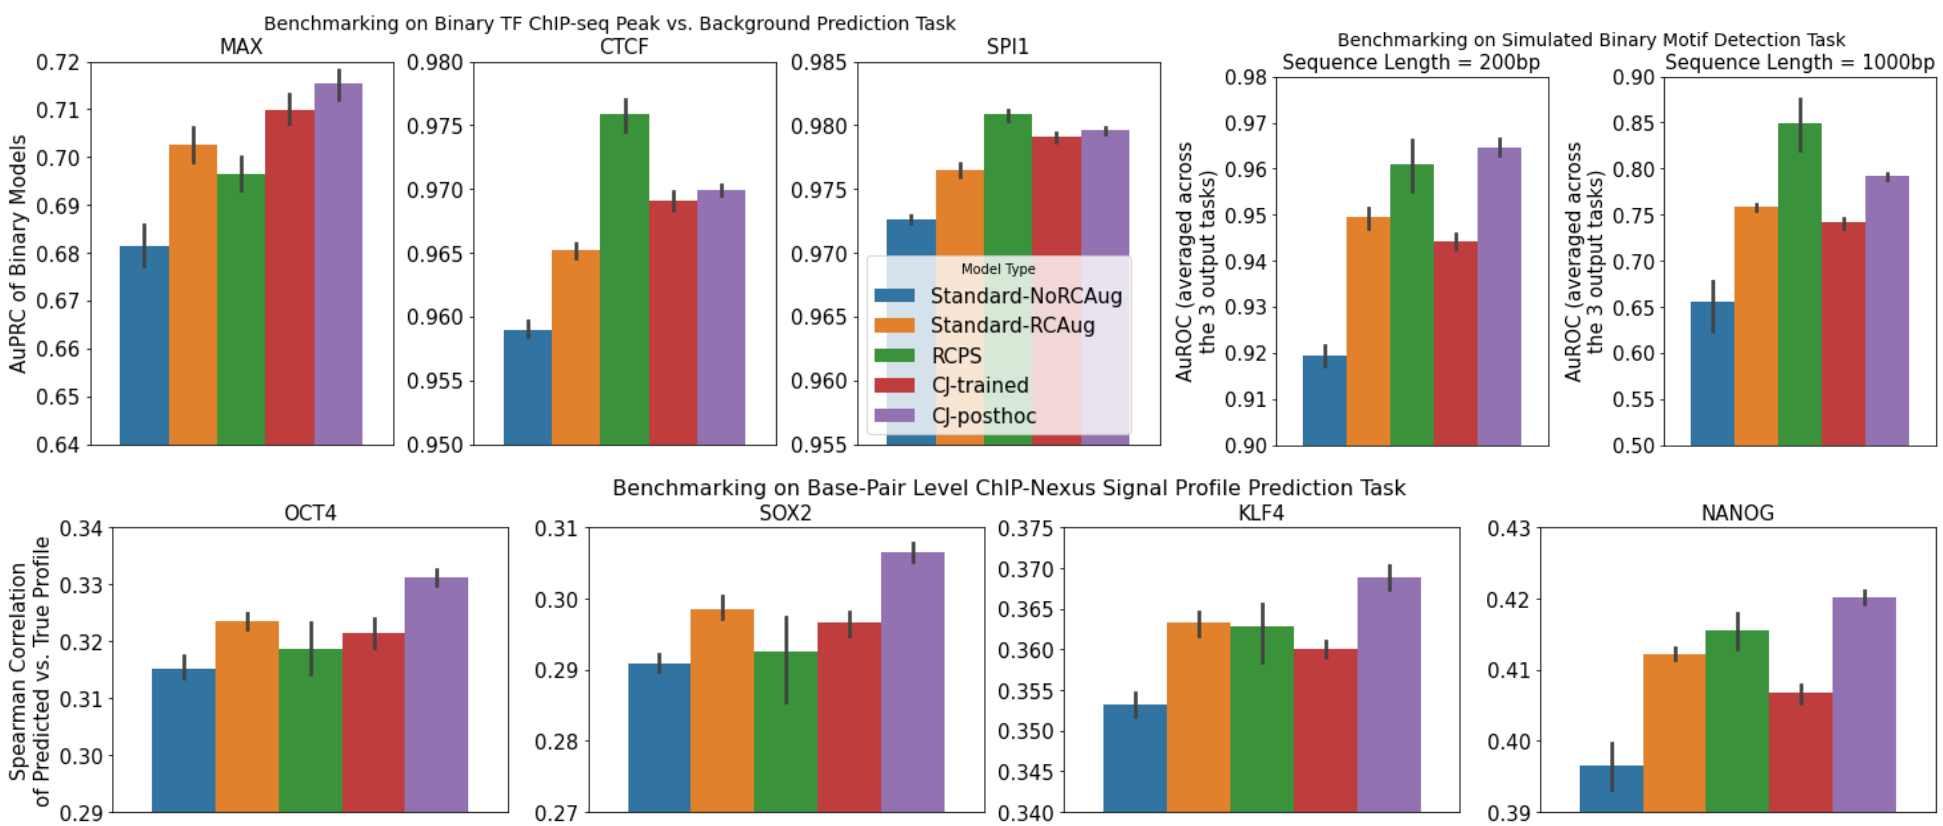
\includegraphics[width=\textwidth]{zhou_equivariance.png}
	\caption{The RC-augmented(RC-aug), RCPS, conjoined (CJ-trained), and conjoined post-hoc (CJ-posthoc) models were evaluated on ChIP-seq, ChIP-nexus, and simulated datasets. Figure adapted from \cite{zhouBetterUnderstandingReverseComplement2021}}
\end{figure}

\subsection{Canonicalization}
Canonicalization offers a third strategy for handling symmetries,
distinct from both data augmentation and architectural weight-tying.
Instead of forcing invariance within the network (as in RCPS) or
implicitly teaching it through the data (as in RC-aug), canonicalization
transforms the input to a standard orientation before it enters the
model so that the network never needs to explicitly learn or impose the
symmetry.

Before \cite{kabaEquivarianceLearnedCanonicalization2023}, other frameworks were proposed in specific and
non-generalized forms, such as spatial transformer networks
\citep{jaderbergSpatialTransformerNetworks2015}. \citet{kabaEquivarianceLearnedCanonicalization2023} formalizes
and generalizes this approach, making the model \(\phi(x)\) be: \[
\phi(x)=h'(x)\cdot f\left( h^{-1}(x)\cdot x \right) 
\] Where:
\begin{itemize}
	\item \(h(x)\) predicts the transformation that the canonical
	version of \(x\) underwent, and its inverse is taken to bring \(x\) to
	its canonical version
	\item \(f(x)\) is the prediction function 
	\item \(h'(x)\)
	predicts the transformation that the \(y\) of that canonical \(x\)
	underwent. On RC-invariant tasks, $h'(x)$ is the identity function for all $x$
\end{itemize}

\begin{figure}[H]
	\centering
	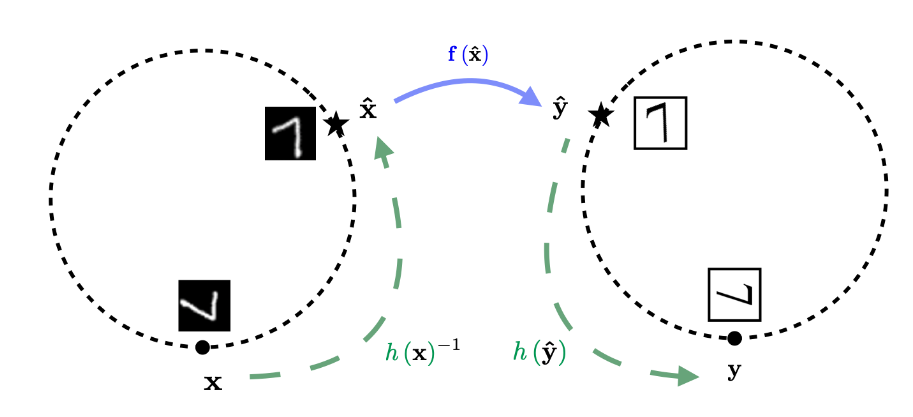
\includegraphics[width=0.5\textwidth]{kaba.png}
	\caption{A diagram of the canonicalization process for a task where the goal was to recognize MNIST digits' rotation in an RC-equivariant way, where the digit is transformed to its canonical form, recognized, and then the classification is rotated back to its original form. Figure adapted from \cite{kabaEquivarianceLearnedCanonicalization2023}}
\end{figure}

It is important to note that this work uses only the general concept of
canonicalization: transforming the input to a standard orientation
before processing it. It does not adopt the specific techniques that \citet{kabaEquivarianceLearnedCanonicalization2023} propose to make this function learnable end-to-end.

\subsection{ConvNova}
ConvNova \citep{boRevisitingConvolutionArchitecture2025} is a convolutional
network that was evaluated on multiple benchmarks: the Nucleotide
Transformer benchmark\citep{dalla-torreNucleotideTransformerBuilding2025}, Genomic Benchmark \citep{gresovaGenomicBenchmarksCollection2023}, BEND Benchmark
\citep{marinBENDBenchmarkingDNA2023}, and on chromatin profile prediction using the DeepSEA dataset \citep{zhouPredictingEffectsNoncoding2015}, and it outperformed many SoTA models despite having fewer parameters and a lower runtime.

\begin{figure}[H]
	\centering
	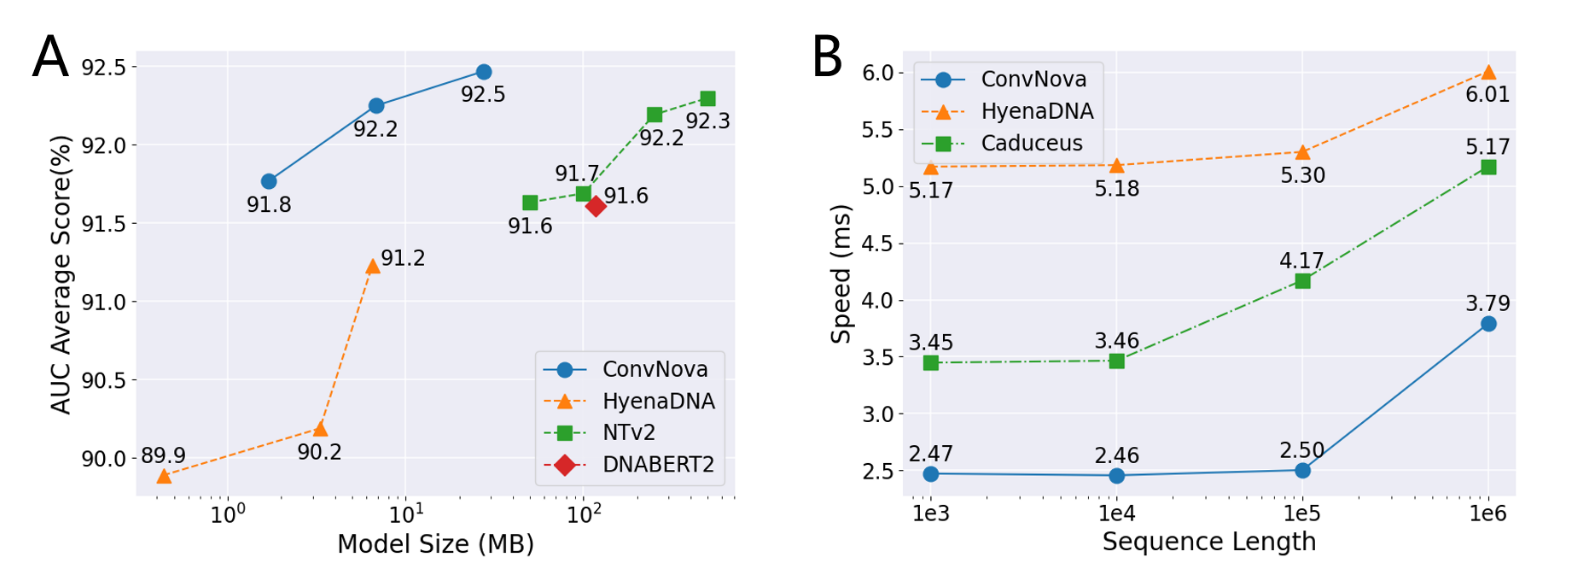
\includegraphics[width=\textwidth]{convnova_performance.png}
	\caption{Trade-off between model performance and size for ConvNova and baseline methods. (A) Performance versus parameter count. (B) Inference time versus sequence length. Figure adapted from \cite{boRevisitingConvolutionArchitecture2025}}
\end{figure}

\subsection{Related work that deal with transcriptional asymmetry}
\label{sec:related_worl_transcriptional_asymmetry}

Based on the available literature, the only works found that deal with the transcription-related asymmetry mentioned previously are:
\begin{itemize}
	\item LegNet\citep{penzarLegNetBestinclassDeep2023}, which adds an additional input channel \texttt{is\_reverse} to the sequence indicating the input strand to deal with the orientation-related asymmetries in regulatory elements.
	\item Asymmetron\citep{georgakopoulos-soaresAsymmetronToolkitIdentification2021}, a toolkit for statistically analyzing strand asymmetries.
\end{itemize}

\section{Methods}

\subsection{Network architecture}
ConvNova was used for the evaluation of the canonicalization's performance, which is a CNN consisting of a series of Gated
Convolution Blocks (GCBs), which consist of a gated convolution
\citep{yuFreeFormImageInpainting2019} with dilated filters
\citep{yuMultiScaleContextAggregation2016}, with an MLP or pooling at
the end depending on the task.

The model takes the DNA and its reverse-complement as inputs
\(\text{A}\) and \(\text{B}\) and computes the output as follows, making
the features of \(\text{A}\) be updated depending on the gating imposed
by \(\text{B}\)
\begin{gather*}
	h=\text{GELU}(\text{convolution}(\text{A}))\\
	g=\text{sigmoid}(\text{convolution}(\text{B}))\\
	\text{A}=\text{A}+h\odot g\\
	\text{B}=\text{B}+g
\end{gather*}

\begin{figure}[h!]
	\centering
	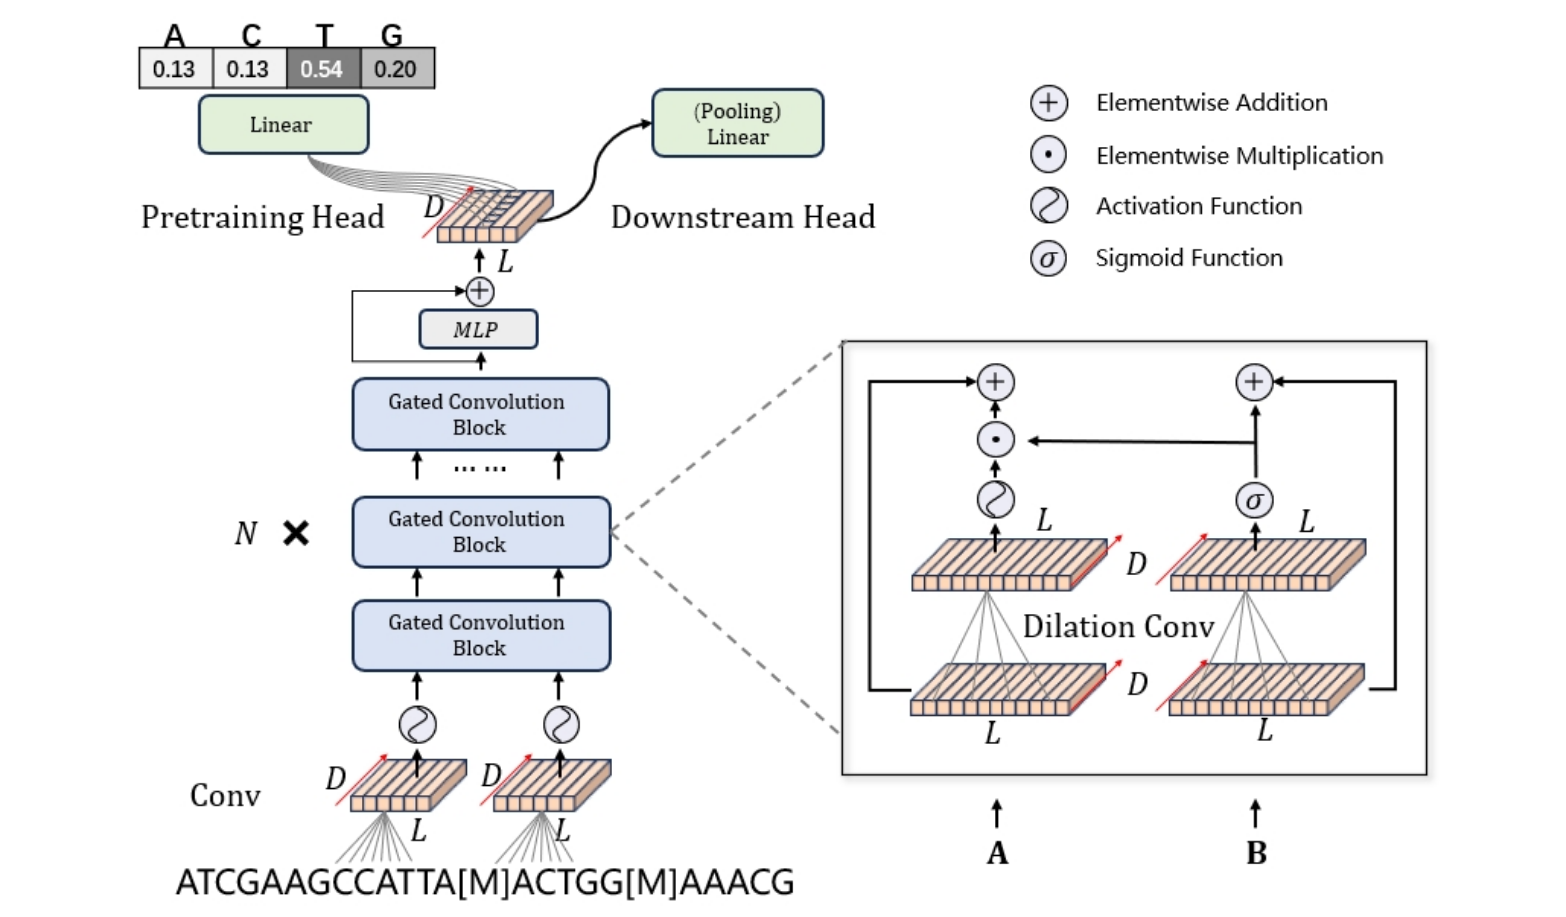
\includegraphics[height=0.3\textheight]{convnova_arch.png}
	\caption{Diagram of ConvNova's architecture. Figure adapted from \cite{boRevisitingConvolutionArchitecture2025}}
\end{figure}

The dilation rate of the GCBs increases as \([1,1,d,d^2,d^3,\dots]\) for
each block. At the end of the series of GCBs, the output \(A\) is passed
through an MLP before being passed to the downstream head.

ConvNova was chosen because it achieves state of the art metrics with a
relatively small number of parameters, because using an RC-invariant or
RC-equivariant architecture would nullify the effect of
canonicalization, and because by taking both DNA strands, it could more
clearly see the asymmetries between the forward and RC strands mentioned
earlier.

\subsection{Canonicalization}

The canonicalization algorithm consists of a pipeline that consists of:
\begin{enumerate}
	\def\labelenumi{\arabic{enumi}.}
	\item Extract all transcribed features (including pseudogenes), their
	positions, and whether they are oriented in coding or template form in
	the dataset. The orientation of the features is obtained directly from
	the `Strand' field.
	\item
	To classify features as transcribed or not: For annotations without a
	standardized type field (NCBI), the Sequence Ontology hierarchy
	\citep{eilbeckSequenceOntologyTool2005} was used to programmatically
	determine which features correspond to transcribed units; for GENCODE
	annotations, the `Feature' and `Transcript type' fields were used
	directly.
	\item
	Based on that, the goal is for all transcribed features (we'll call these \emph{segments} from now on) to be in the coding
	orientation (chosen arbitrarily) by taking the reverse-complement of
	their coordinates in the genome.
	\item
	In the case where there are overlaps between segments of opposite
	orientations, applying RC to one segment is considered to
	\textbf{completely} destroy both segments (this hypothesis produced the best results, see section \ref{sec:methods_optimal_canonicalization_search} for more details). In that case, both segments are left as is.
	\item After the whole genome is canonicalized, it's then saved and the model is trained on it
\end{enumerate}

Multiple canonicalization algorithms were evaluated. For details on the different algorithms, see section \ref{sec:methods_optimal_canonicalization_search}, and for more details on the different algorithms evaluated and section \ref{sec:methods_evaluation_canonicalizaiton_algorithms} for the evaluation protocol.

For the downstream tasks, their DNA sequences are aligned, using
minimap2 (\citep{liMinimap2PairwiseAlignment2018}) in the case where the
coordinates are not given and only the sequence is available along with
the genome from which they were taken. We refer to this genome as the
source genome, and this alignment is performed to determine whether the
sequences fall on a transcribed feature and must be canonicalized.

If more than 50\% of the sequence must be transformed, then the entire sequence is transformed along with its label. The basis of this algorithmic decision is arbitrary. Both this method and a simpler one that just canonicalizes every transcribed part of a sequence yield the same results with a negligible difference, matching the results discovered on the hyperparameter search (see section \ref{sec:hyperparameter-optimization-results}), which argues in favour of the hypothesis that partial canonicalization breaks the whole sequence (see section \ref{sec:design-of-the-canonicalization-algorithm}) 

The label transformation method depends on the tasks, and they are divided into 3 categories:
\begin{itemize}
	\item RC-invariant tasks where the target value of \(S\) is the same as \(RC(S)\) 
	\item RC-equivariant tasks where the target values are not
	equal, but the target value of \(RC(S)\) can be known from that of \(S\)
	\item Tasks where the label of \(RC(S)\) can only be known by obtaining
	experimental data. In these cases, canonicalization is skipped for the
	entire task (since transforming the sequence would break the label)
\end{itemize}

Regions without transcribed segments remain unmodified and passed in arbitrarily as they were on the origin genome, as done in ConvNova. Even if the
sequence falls on the negative strand and the model never saw it, I will
not take its RC in order to test the model's generalization.

It should also be noted that not all transcribed segments are
canonicalized, since when there are overlaps, the canonicalization
algorithm has to make compromises in certain places. Even so, it is
assumed that all segments were canonicalized correctly, since the goal
is to evaluate how well the model learns to capture transcriptional
asymmetries, not the compromises the canonicalization algorithm had to
make.

\subsection{Evaluation of the canonicalization algorithm}
\label{sec:methods_evaluation_canonicalizaiton_algorithms}

To evaluate the canonicalization method (described more extensively below) the training data is
pre-processed, and the same pretraining and fine-tuning protocol 
in the ConvNova paper is used (except for the cases where it is
explicitly stated that a different protocol was used)

For each of the tasks, as with ConvNova, the model is pretrained on hg38
using MLM. 10\% of the nucleotides are masked and the model's objective
is to predict the masked nucleotides.

For the downstream tasks, simply comparing the performance of the non-canonicalized model vs the canonicalized one isn't enough, because the canonicalization algorithm uses additional data, introducing a data leakage that could be inflating the true improvement caused by the canonicalization algorithm.

In the gene finding task from the BEND Benchmark, for example, a task that
consists of classifying each nucleotide as exon, intron, acceptor,
donor, or nothing, the (noisy) introduction of the strand orientation data by the canonicalization algorithm produces a leakage.

To mitigate that, an ablation was designed where 3 different versions of the model are evaluated:
\begin{itemize}
	\item Baseline: The baseline model without any canonicalization
	\item Canonicalized: The model evaluated on the canonicalized datasets
	\item Leakage control: The model evaluated on the non-canonicalized datasets with an extra channel on its input indicating whether that nucleotide is a positively transcribed feature (+1), a negatively transcribed feature (-1), or isn't transcribed (0)
\end{itemize}

The evaluation protocol for a model consists of 5 runs with 5 different random seeds. Those 3 versions of the model are evaluated using that protocol on all downstream tasks using a fewer-parameter configuration to speed up the evaluation (see section \ref{hyperparameter-search}).

Then, for the tasks where a promising difference appears between the canonicalization model vs the baseline and leakage control models, that same evaluation protocol is used but with the original, larger configuration used in ConvNova. This screening step is only used to decide which tasks deserve the additional compute of a full-scale evaluation.

The criterion for deciding if an observed difference between the canonicalized model and the other two models is promising is by computing the right-tailed p-values for the canonicalized model vs the baseline, and the canonicalized model vs the leakage control one, taking the largest of those p-values, and checking if they're low or not.

It's worth noting that for the leakage control model, because of the additional input channel, has slightly more parameters than the baseline and canonicalized models. The difference is under 0.5\% in relative terms and is therefore negligible.

The 5 random seeds used were: 1938, 205, 8262, 1480 and 4436.

\subsection{Downstream tasks}
For the choice of baselines and evaluation protocol, the protocol established by the authors of ConvNova
\citep{boRevisitingConvolutionArchitecture2025} will be followed, unless stated
otherwise. The reason this protocol was used is that, by using ConvNova
as the architecture and only changing the data pre-processing, the
results are directly comparable.

All models were fine-tuned after being pretrained on hg38. For details
regarding how the labels of each downstream task were handled, see
section \ref{sec:downstream-task-canon-classification}. The downstream tasks and their details are listed below. Each downstream task has a specific model configuration, see section \ref{sec:appendix_downstream_tasks} for more details.

\subsubsection{NT Benchmark} 
This benchmark is the one used by Nucleotide Transformer
(\cite{dalla-torreNucleotideTransformerBuilding2025}). It consists of 3
types of tasks: histone marker prediction, splice site annotation
prediction, and regulatory annotation prediction. It should be noted
that the most recent version of the benchmark was used, which was not
used in the original ConvNova paper.

To evaluate the tasks, the same methodology as in HyenaDNA
(\citep{nguyenHyenaDNALongRangeGenomic2023}) was followed, using the
Matthews Correlation Coefficient (MCC) for certain tasks and the
F1-score for others. The results of the model with canonicalization are
compared against the model without canonicalization, and the rest of the
models against those the original ConvNova paper compared against.

For canonicalization, GRCh38 was used as the source genome and the
annotations were obtained from the Genome Reference Consortium, since all the datasets come from human samples. The tasks were evaluated using a pooling downstream head.

\subsubsection{Genomic Benchmark}
It is a multi-species benchmark, consisting of human, mouse,
roundworm, and fruit fly samples. Its tasks consist of enhancers,
species classification, and regulatory elements.

For canonicalization, the following source genomes were used: hg38 for
the human sample tasks, GRCm39 from the Genome Reference Consortium, and for the roundworm and drosophila sample
tasks the NCBI reference genomes were used. The tasks were evaluated using a pooling downstream head.

Keep in mind that for \texttt{human\_ensembl\_regulatory}, the model performance dropped compared to the original ConvNova paper because a longer sequence length was used, where the whole dataset sequence is passed to the model instead of a trimmed version of it like in the original ConvNova paper (see more details in section \ref{sec:appendix_downstream_tasks}). It's theorized that this happens because of the pooling decoder diluting the signal located at the start of the sequence used for prediction.

\subsubsection{BEND Benchmark}
The model was evaluated only on the gene finding tasks, where given a DNA sequence
each nucleotide must be classified as intron, exon, or neither, and CpG
methylation, where given a DNA sequence multilabel classification is
performed on whether it is methylated or not in different cell lines.

The chromatin accessibility and histone modification tasks are redundant
compared to the tasks in the rest of the benchmarks, and therefore were
not included in the evaluation.

The zero-shot variant effects tasks were also skipped, since unlike
models with an attention mechanism, each output token was determined by
a very small local context, and if one wanted to mitigate that through
pooling, the SNP token signal becomes too diluted for classification.
Evaluating those tasks in that way gives artificially low results.

For CpG methylation a linear head was used over the entire encoded
sequence, and for gene finding each token is passed through a linear
layer.

\subsubsection{Chromatin Profile Prediction}
This task \citep{zhouPredictingEffectsNoncoding2015} consists of predicting
chromatin profiles and epigenetic markers given a DNA sequence. The
dataset consists of 919 chromatin features, grouped into transcription
factor binding profiles, DNase I hypersensitivity, and histone marks.

The source genome of DeepSEA is hg19. In this specific case, for
canonicalization, hg38 is used as the source genome in order to use the
most up-to-date annotations, and the coordinates are resolved directly
by aligning the DeepSEA sequences with minimap2
\citep{liMinimap2PairwiseAlignment2018} instead of using the GENCODE
lift-over.

\subsection{Optimal canonicalization parameters search}
\label{sec:methods_optimal_canonicalization_search}

The canonicalization pipeline and its parameters were optimized using Optuna \citep{akibaOptunaNextgenerationHyperparameter2019} using its default TPE optimizer. 20 trials were run to optimize the following parameters:

\begin{itemize}
	\item \texttt{annotations\_level}: Filter the GENCODE annotations to use up to level 1 (validated), 2 (manually annotated), or 3(automatically annotated).
	\item \texttt{transformation}: Whether to transform a feature (and the
	overlaps window) by taking the RC, the complement, or
	inverting it. The optimal value was to take the RC.
	\item \texttt{overlap\_transformation\_behavior}: When encountering a segment $A$ that overlaps with another segment $B$ in the opposite orientation, this variable controls the expected behavior of transforming $A$:
	\begin{enumerate}
		\item If \texttt{overlap\_transformation\_behavior} is set to \texttt{partial break}, then it's believed that only the overlapping part between A and B breaks
		\item If \texttt{overlap\_transformation\_behavior} is set to \texttt{full break}, then it's believed that the \emph{whole} $B$ segment breaks, and it's chosen whether to transform $A$ or transform $B$ depending on other variables. See section \ref{sec:design-of-the-canonicalization-algorithm} for more details
		\item If \texttt{overlap\_transformation\_behavior} is set to \texttt{both break}, then it's believed that both $A$ and $B$ break. Neither segment is canonicalized and they're left as-is.
	\end{enumerate}
	
	\item \texttt{include\_cvdj\_segments}: Whether to count the
	cvdj segments of the human and mouse adaptive immune system as
	transcribed features or not.
	\item \texttt{include\_pseudogenes}: Whether to count pseudogenes or not as transcribed.
\end{itemize}

See section \ref{sec:hyperparameter-optimization-results} for the values chosen for these hyperparameters and more details on the HPO results, and section \ref{sec:design-of-the-canonicalization-algorithm} for more details on the variables used and a more detailed explanation on the different canonicalization algorithms and the way they deal with overlapping segments.

Only 20 trials were used because, even though the number of possible configurations (180) is much larger than the 20 trials used, most of the hyperparameters had very little importance, the improvements were starting to become marginal, and compute was limited. See section \ref{sec:hyperparameter-optimization-results} for more details on the results. It should also be noted that some of the variables are conditioned by others (see section \ref{sec:design-of-the-canonicalization-algorithm}).

To speed up the trials, the model was pretrained and fine-tuned with a
single configuration, in order to obtain representative metrics for the
configuration without having to wait too long. See section
\ref{hyperparameter-search} for more details on the model configuration.

Each trial was evaluated on all the downstream tasks, and its score was computed by averaging the z-score across those tasks. The mean and variance for those z-scores were obtained from the non-canonicalized baseline previously mentioned on section \ref{sec:methods_evaluation_canonicalizaiton_algorithms}. 

Even though there is a considerable task-type imbalance (there are many more histone-marks-related tasks than splicing-related tasks, for example), because there is little to no correlation between tasks, the score for each trial was obtained by simply averaging the z-scores for all tasks.

\begin{figure}[h]
	\centering
	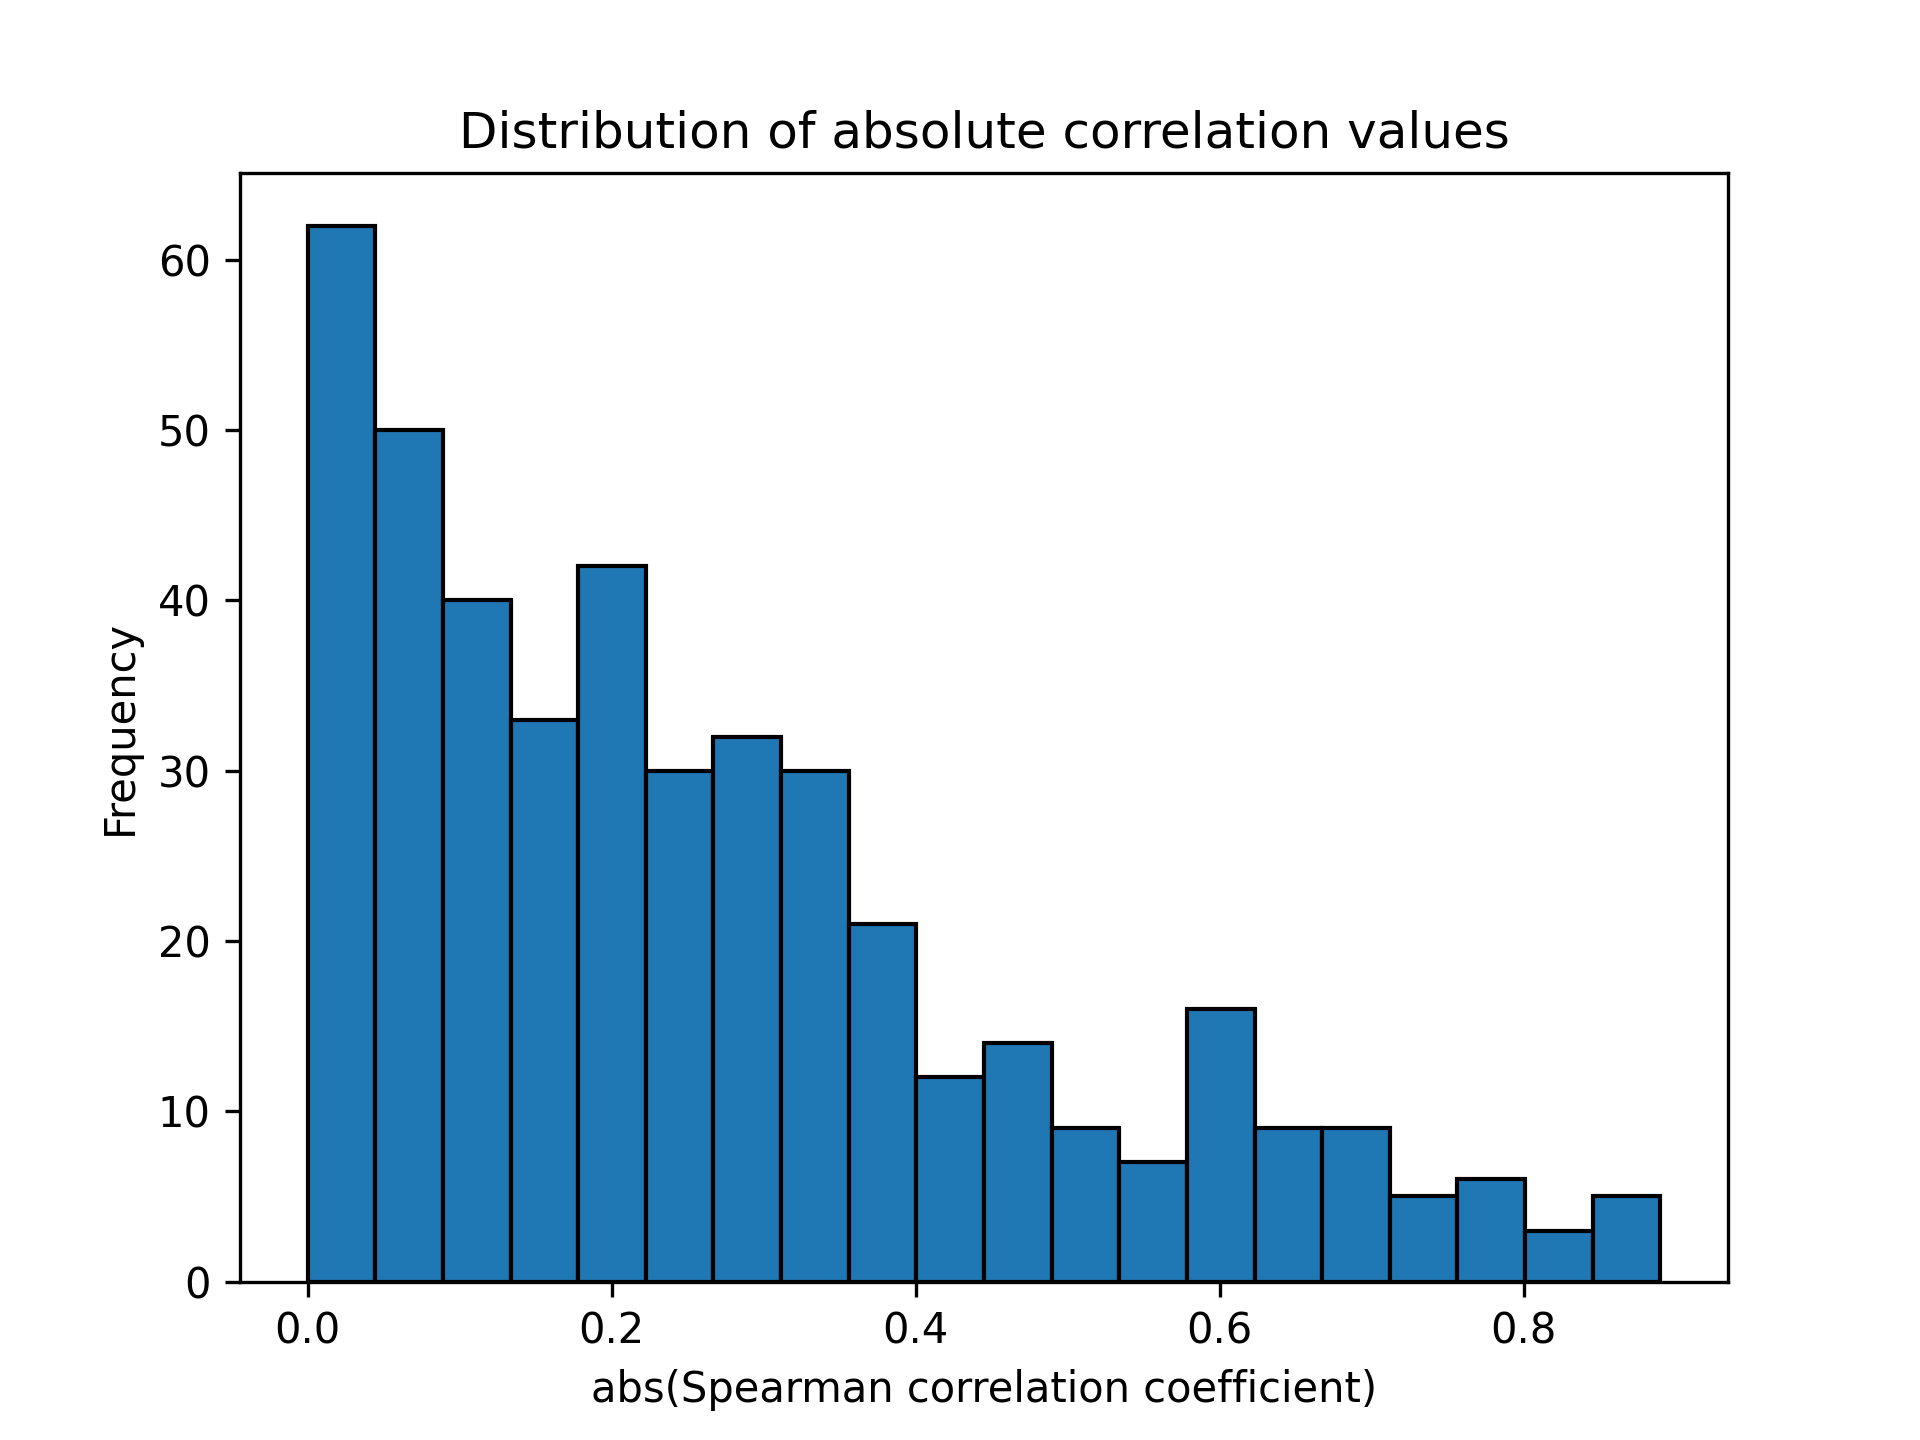
\includegraphics[width=0.5\textwidth,height=0.35\textheight,keepaspectratio]{charts/tasks_correlation_histogram.png}
	\caption{Distribution of the absolute values of the upper triangular section (without including the diagonal) of the Spearman correlation matrix of the downstream tasks.}
	\label{fig:tasks_correlation_histogram}
\end{figure}

\section{Experiments}

\subsection{Comparison between the baseline, canonicalized and leakage control models}

As it can be seen on figures \ref{fig:ablation} and \ref{fig:ablation_p_values}, barely any tasks show a statistically promising difference, and even among those that do the effect size is weak, except for \texttt{demo\_human\_or\_worm}. Still, it was hypothesized that the difference between tasks may increase noticeably when evaluated on the full-scale model. The tasks chosen were: \texttt{H3K4me3, H4K20me1, enhancers, enhancers\_types} and \texttt{demo\_human\_or\_worm}. The results can be seen on table \ref{tab:paper_repeats}.

% --- Primera mitad (superior) ---
\begin{figure}[H]
	\centering
	\makebox[\textwidth][c]{%
		\begin{adjustbox}{width=1\textwidth, trim={0 {0.49\height} 0 0}, clip}
			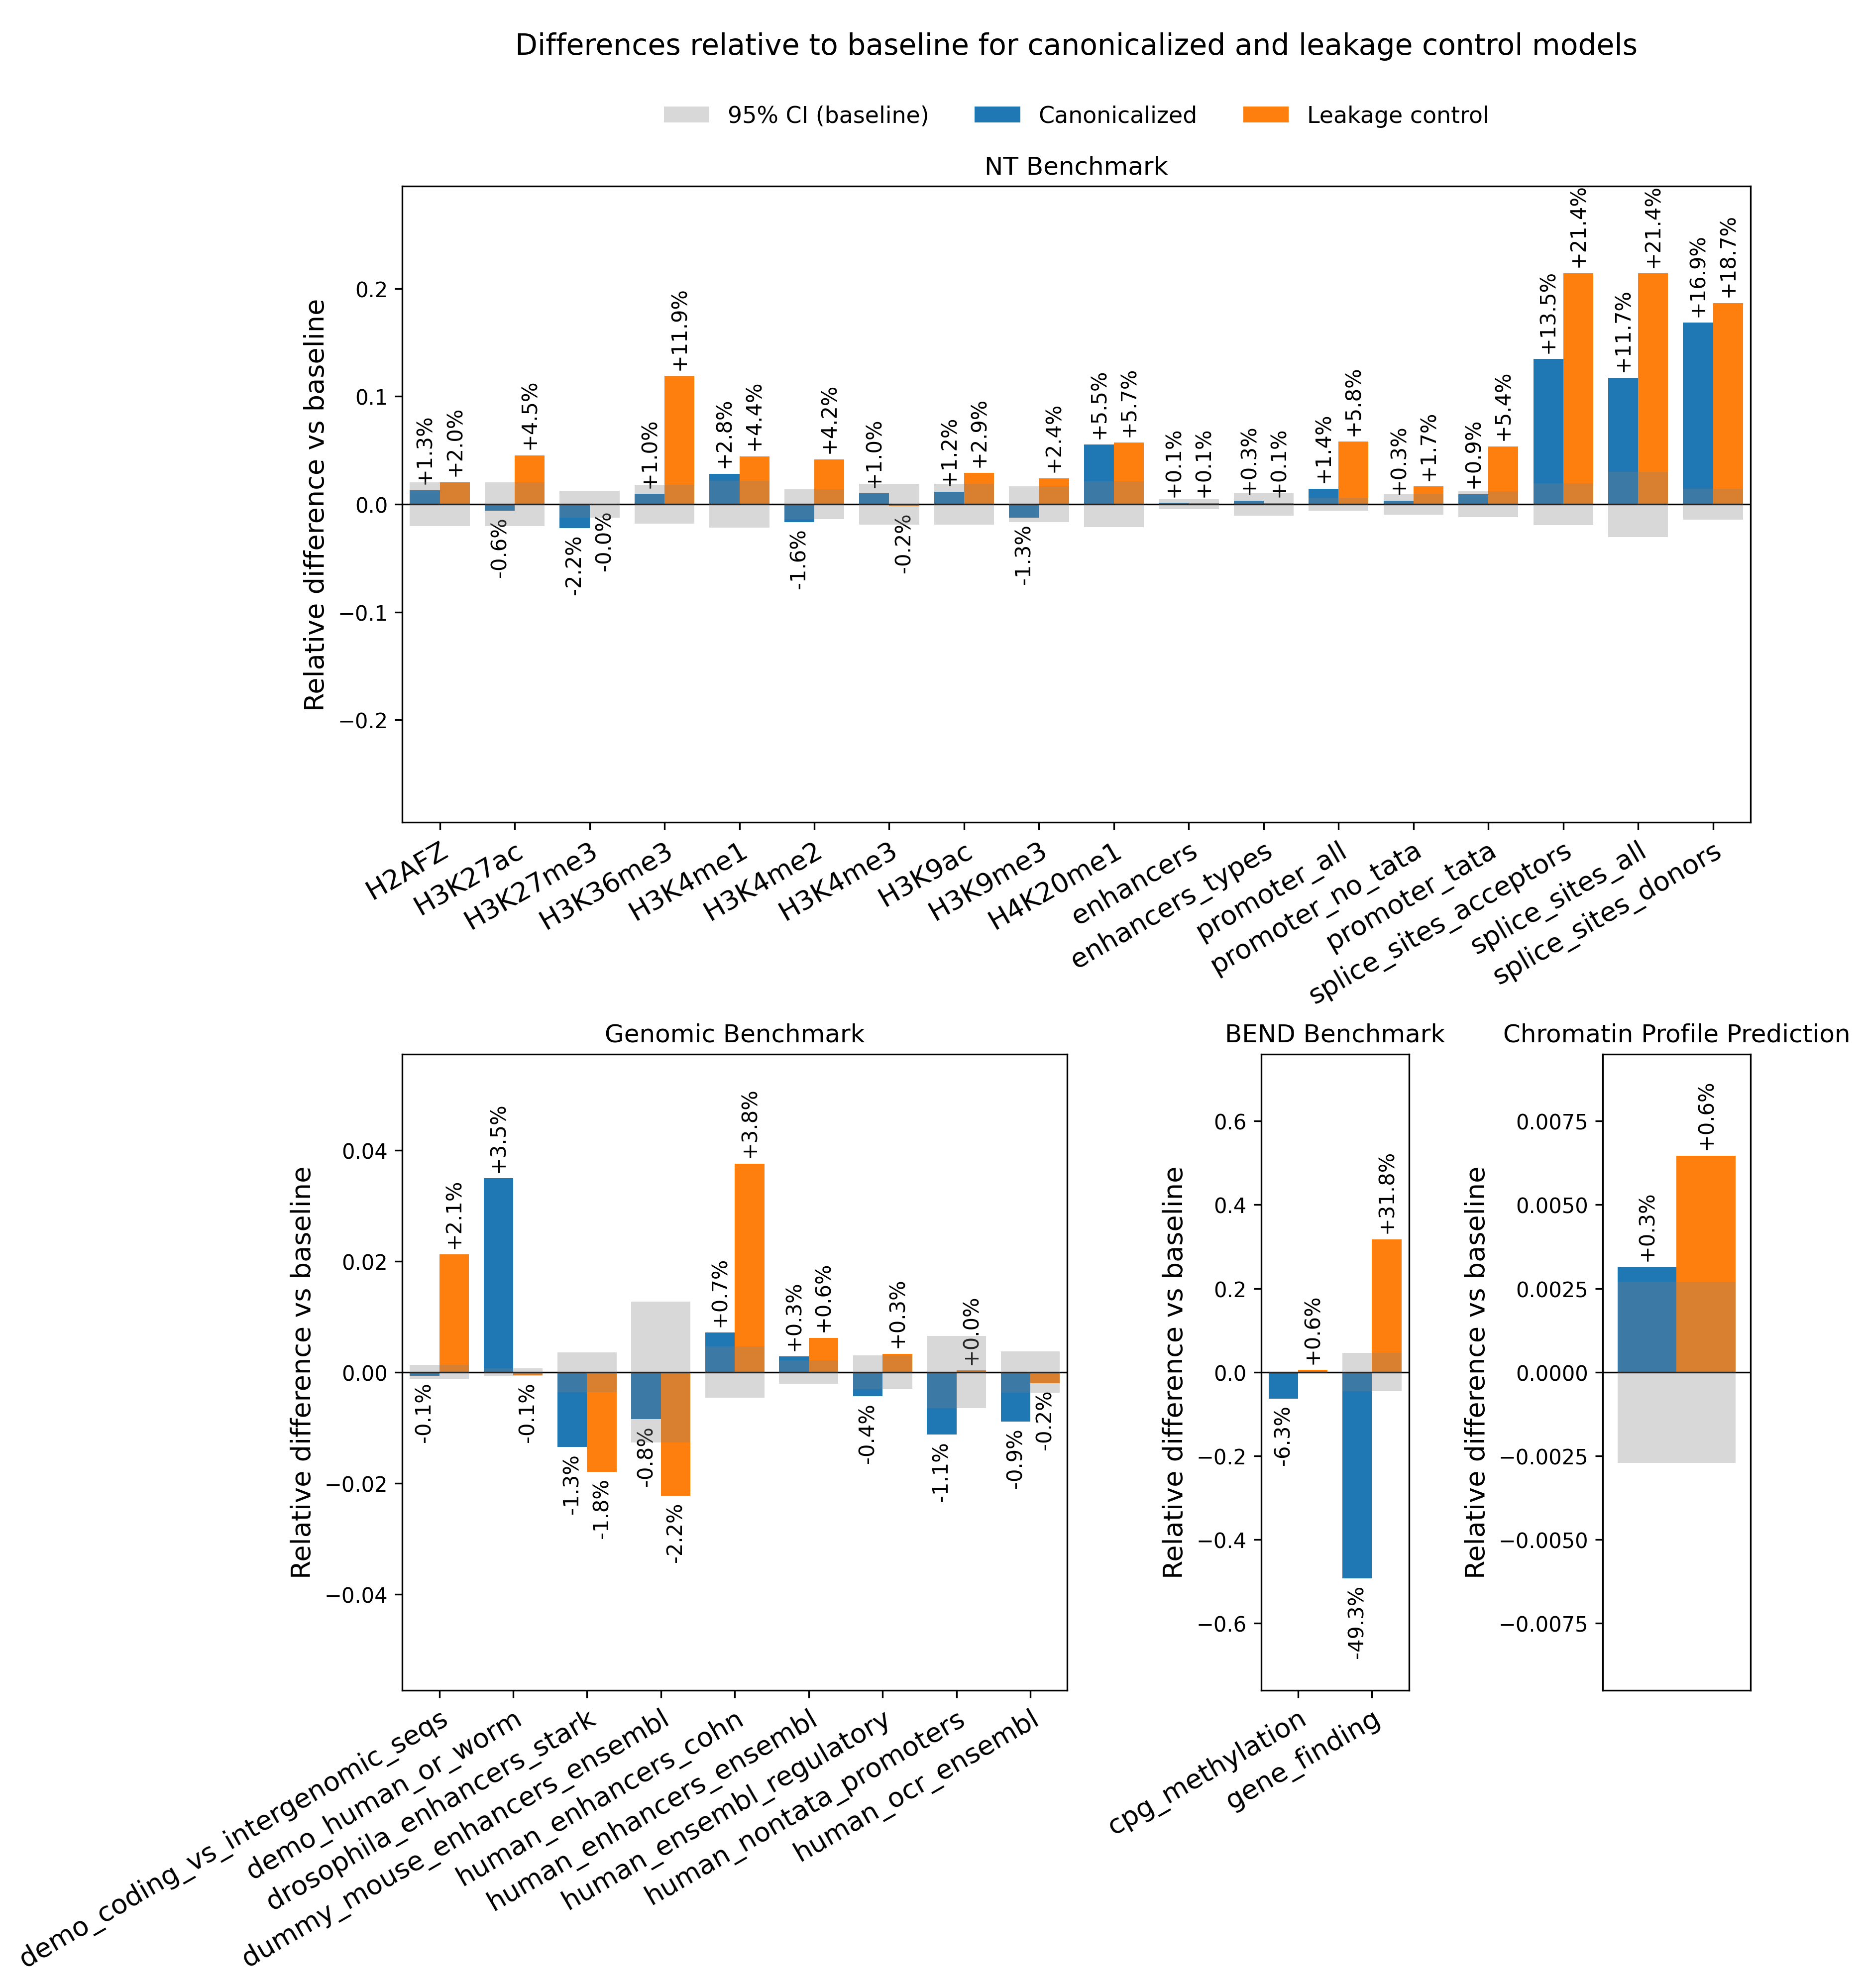
\includegraphics{charts/ablation.png}
		\end{adjustbox}
	}
	\caption*{Upper half of figure \ref{fig:ablation}}
\end{figure}

%\clearpage % opcional, si querés forzar el salto de página acá

% --- Segunda mitad (inferior) ---
\begin{figure}[H]
	\centering
	\makebox[\textwidth][c]{%
		\begin{adjustbox}{width=0.95\textwidth, trim={0 0 0 {0.51\height}}, clip}
			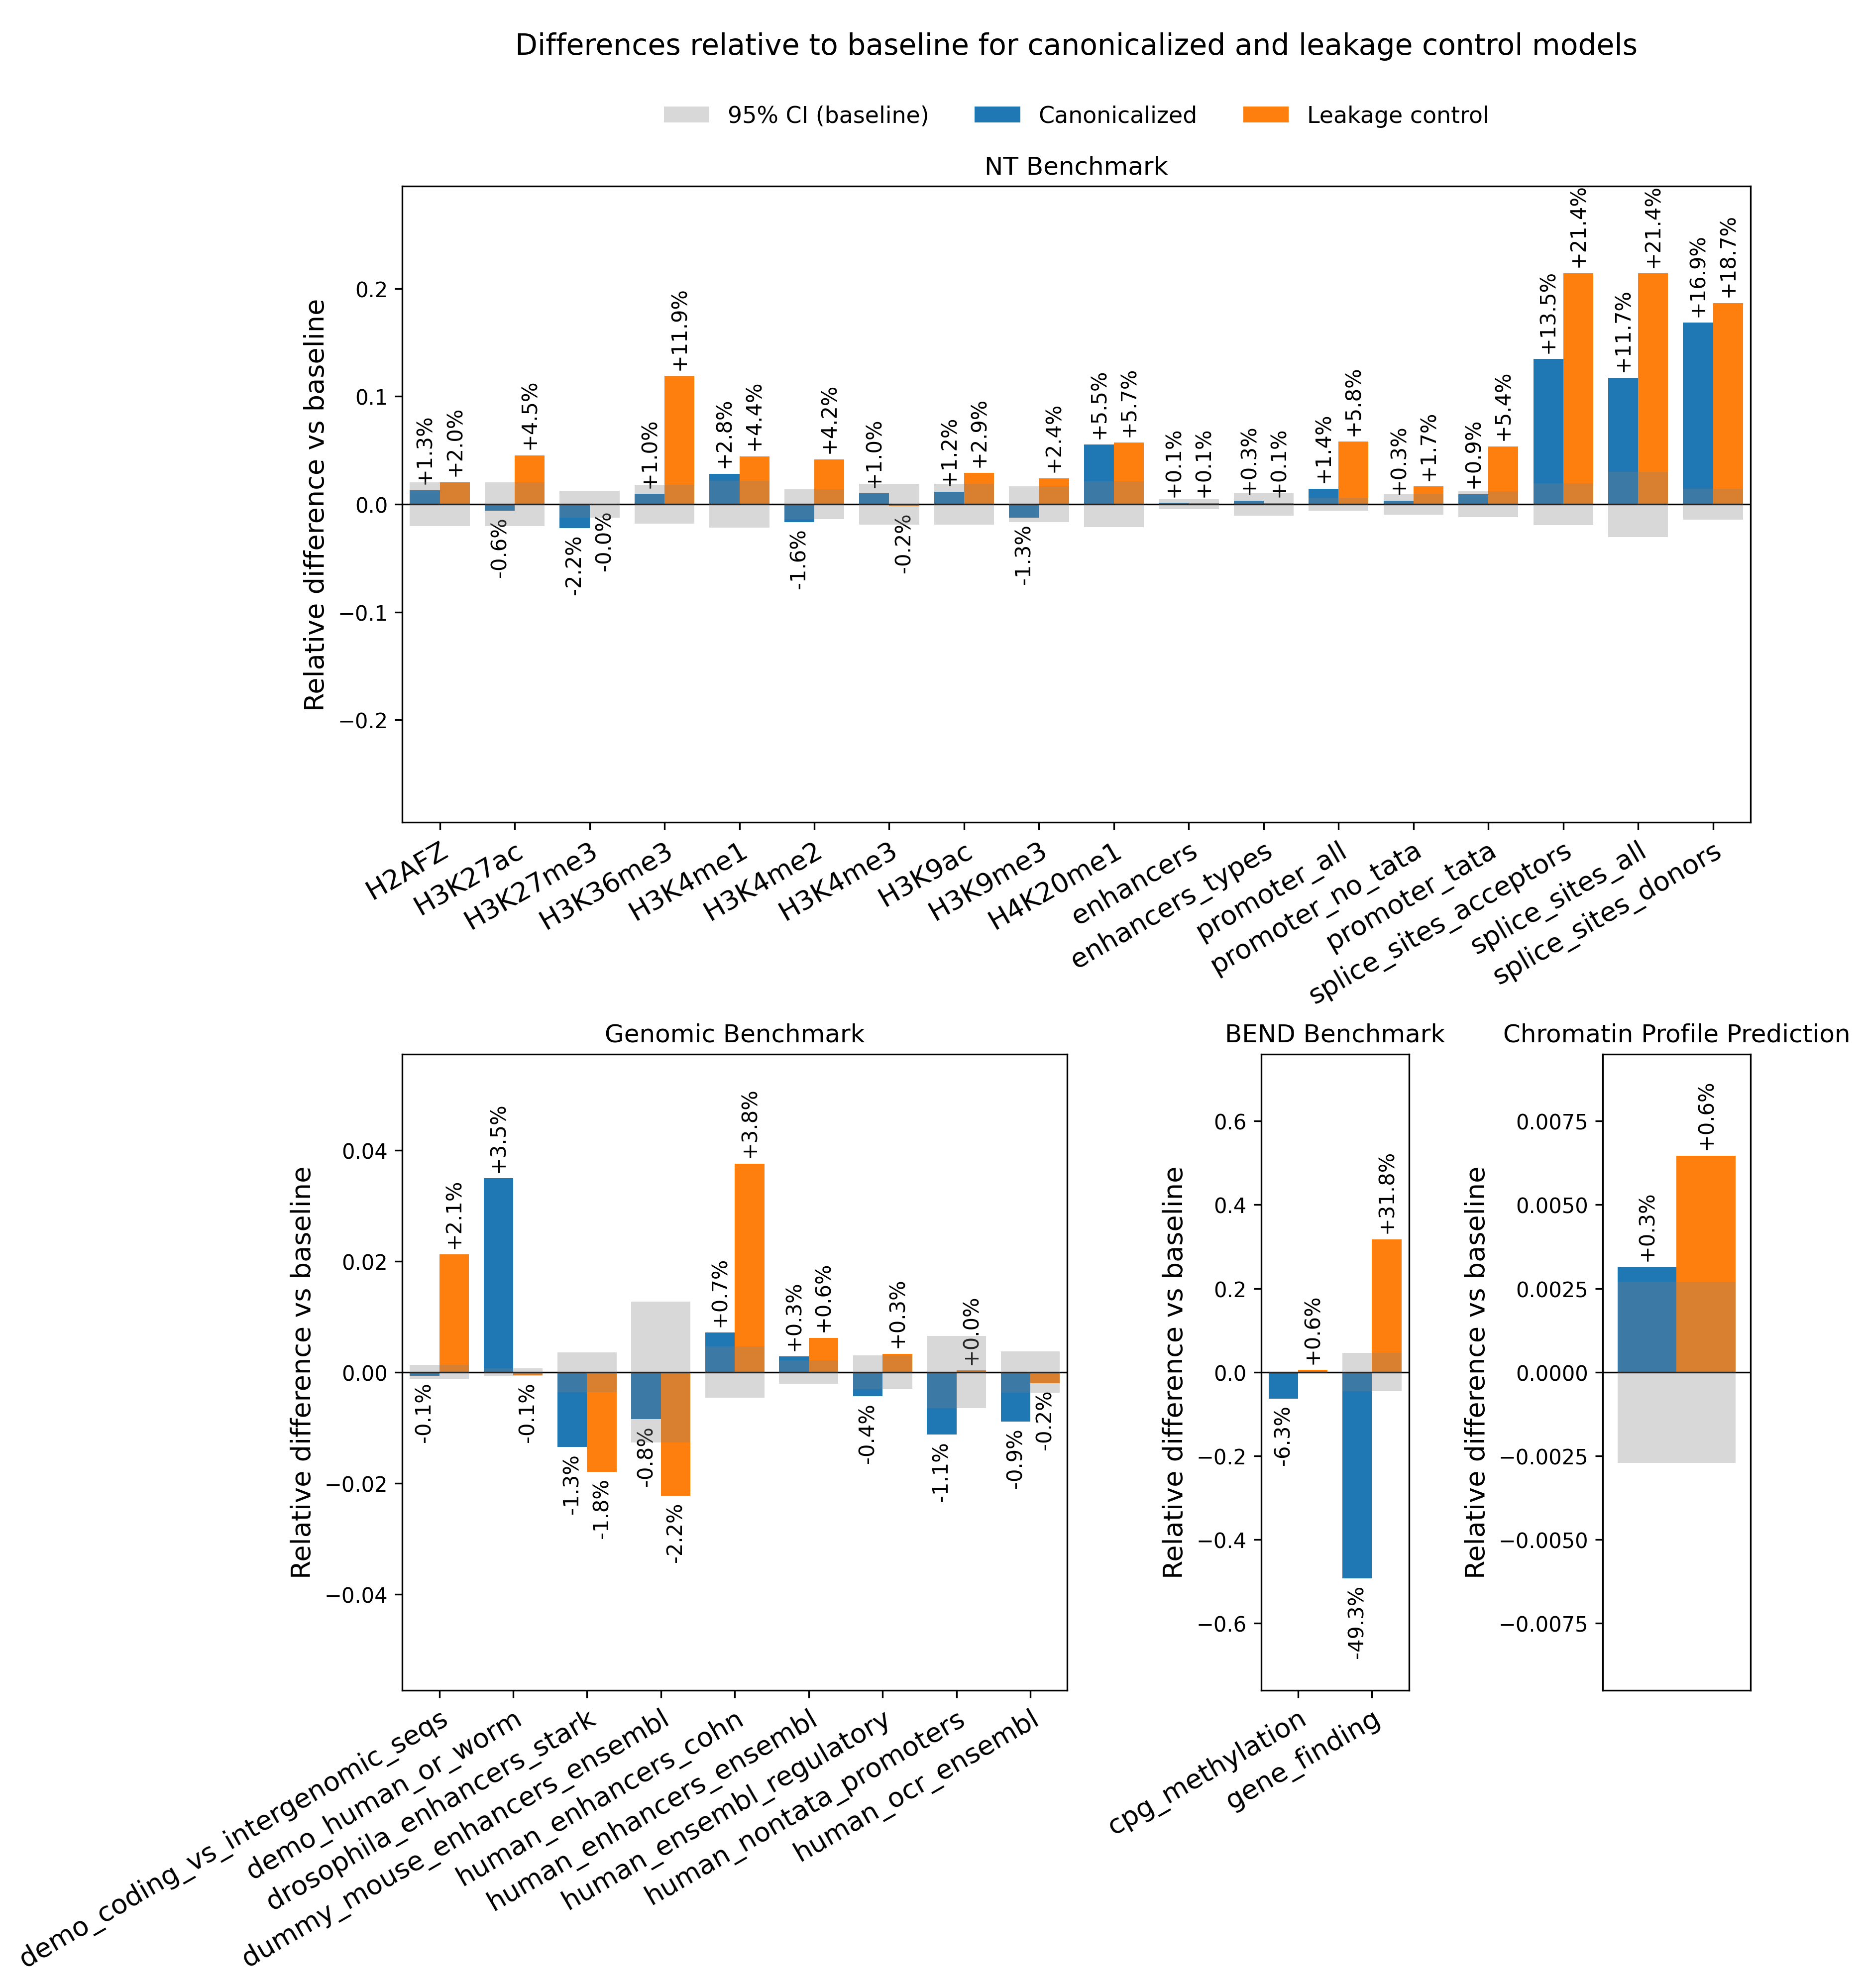
\includegraphics{charts/ablation.png}
		\end{adjustbox}
	}
	\caption{The canonicalized and leakage control mean values with respect to the baseline. The gray area around the baseline represents the 95\% confidence interval for that task. Even though the canonicalized method produces better results than the baseline for most tasks, in the large majority of them, that effect seems to be produced by the data leakage mentioned previously (see section \ref{sec:methods_evaluation_canonicalizaiton_algorithms}) because of the considerable difference between the canonicalized and leakage control methods}
	\label{fig:ablation}
\end{figure}

\vspace{-10pt}

\begin{figure}[H]
	\centering
	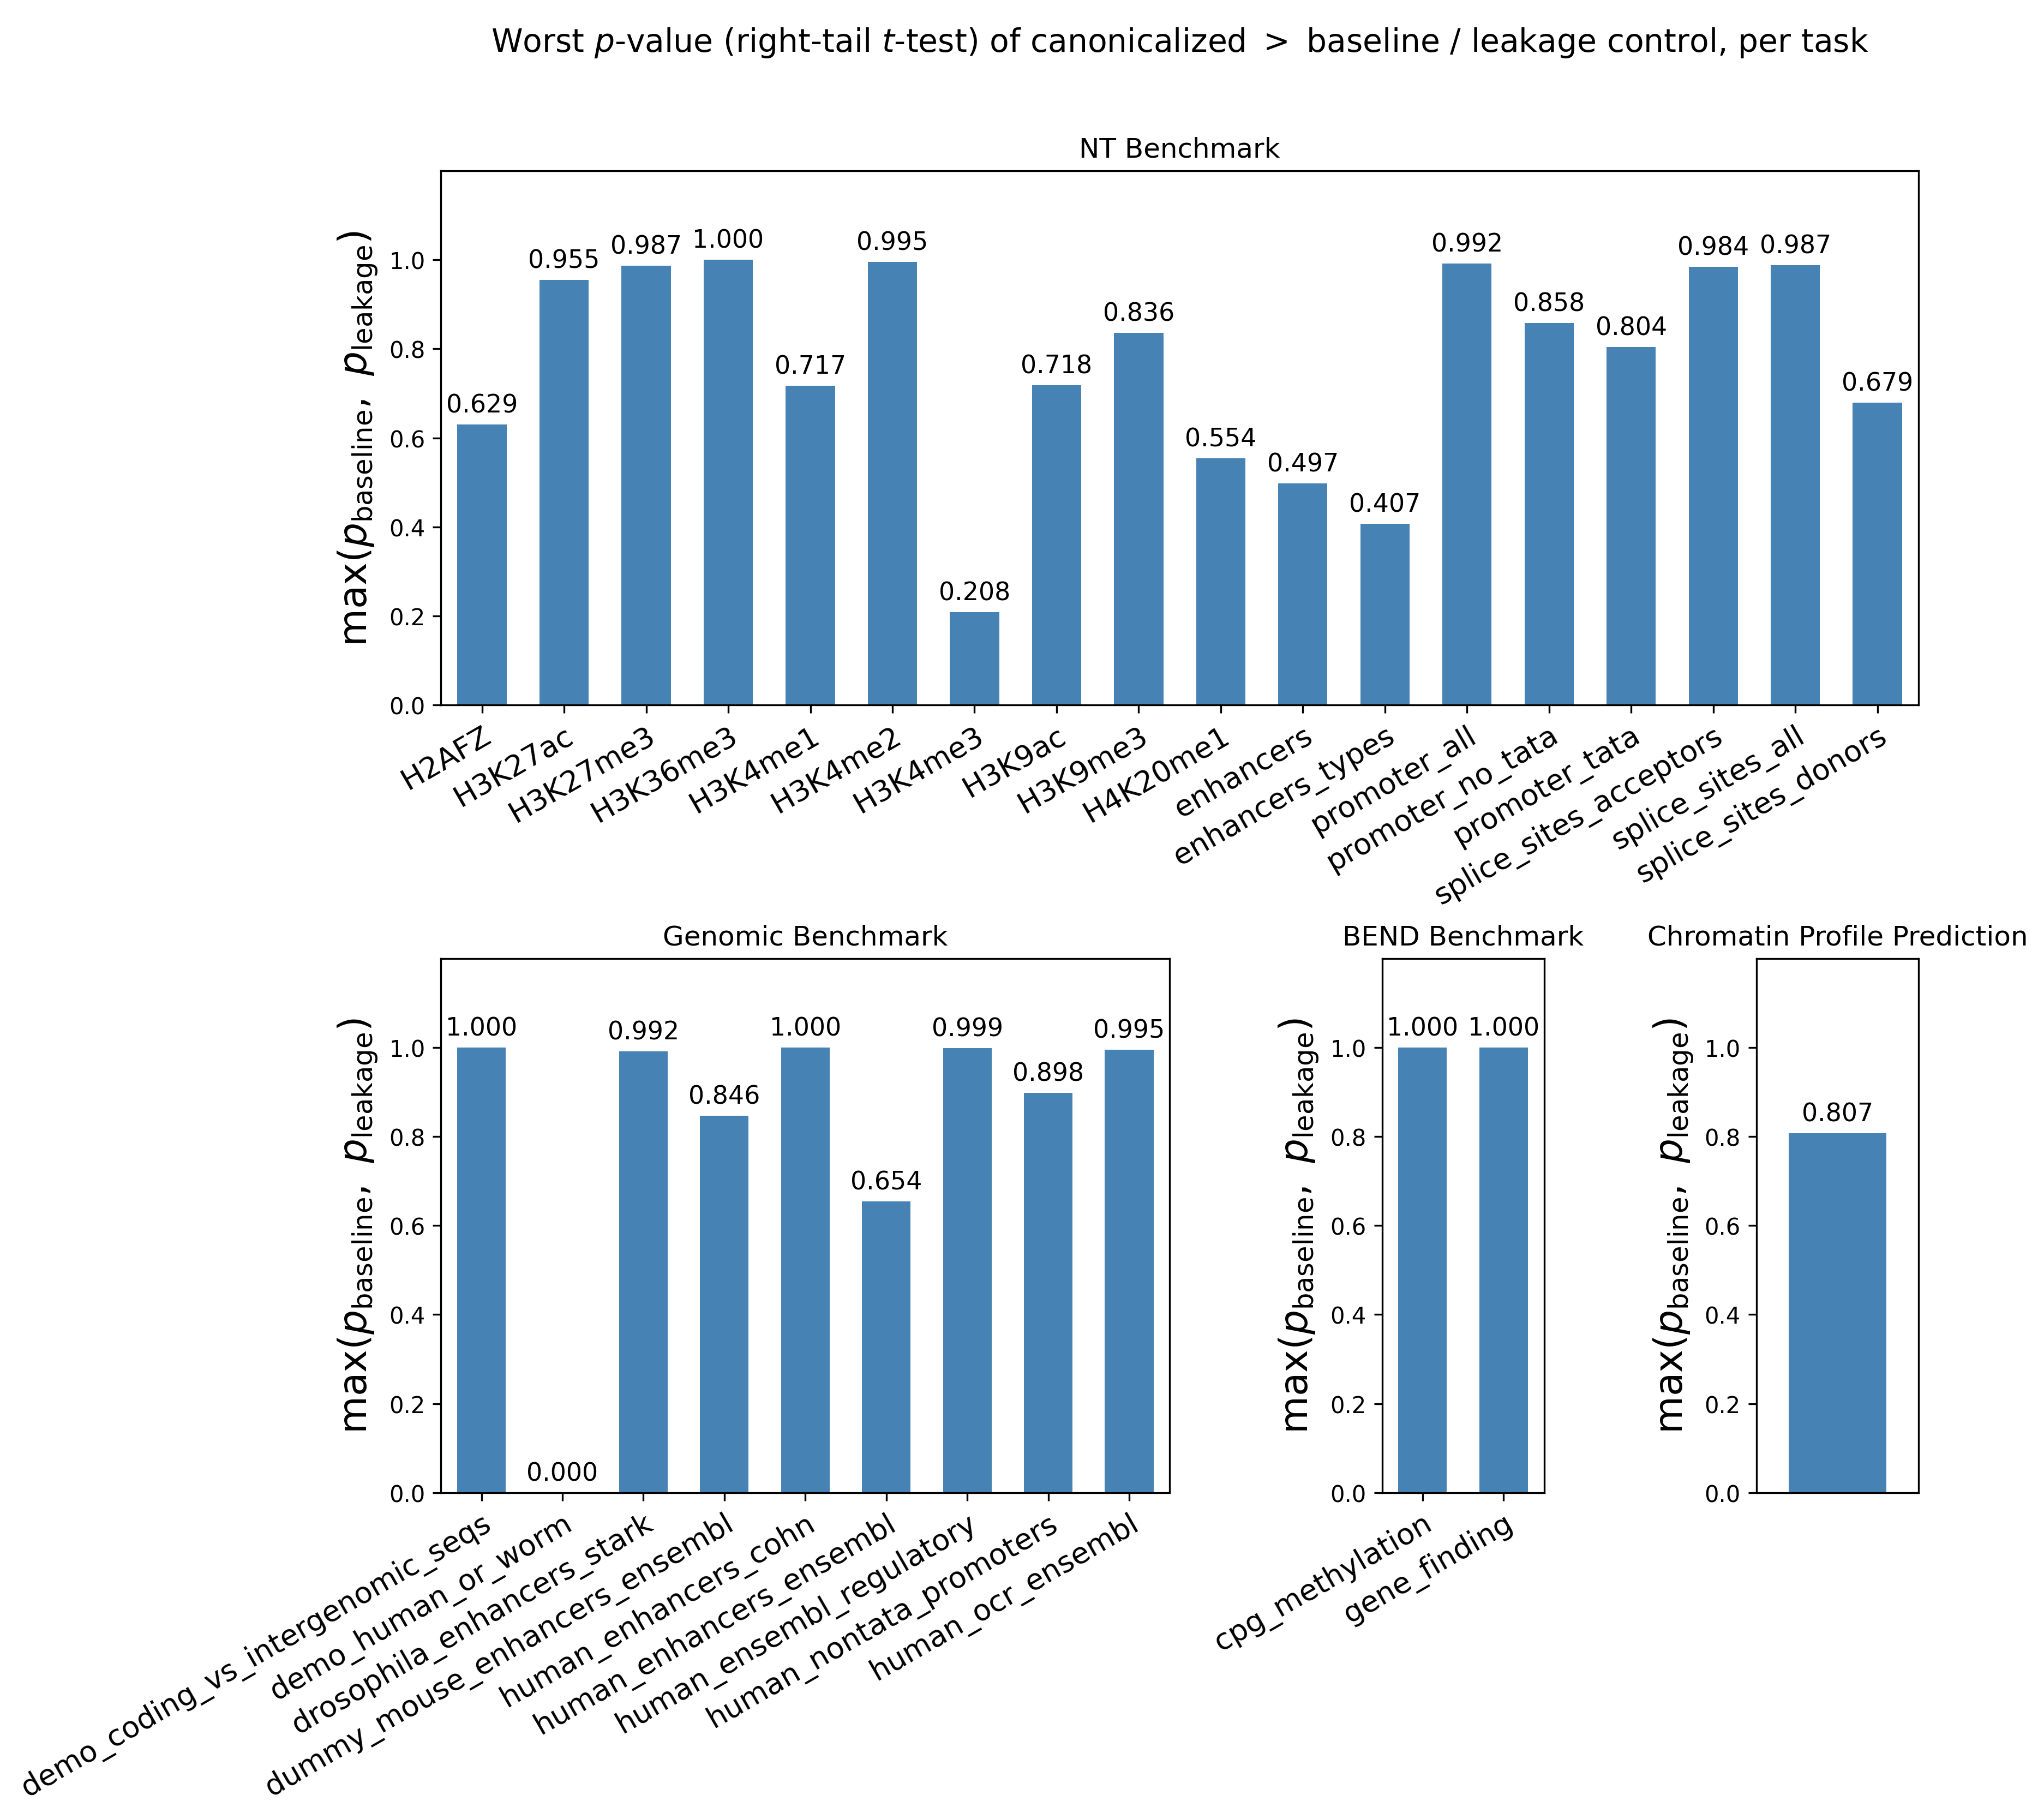
\includegraphics[width=0.91\textwidth]{charts/ablation_p_values.png}
	\caption{The largest of the p-values of $\max(p_\text{baseline}, p_\text{leakage control})$, with both p-values being computed using a right-tailed t-test between the canonicalized having a greater mean than the baseline and leakage control models}
	\label{fig:ablation_p_values}
\end{figure}

\begin{table}[ht]
	\centering
	\begin{tabular}{lcccc}
		\toprule
		Dataset & Baseline & Canonicalized & Leakage Control & $\max\left(p_{\mathrm{baseline}},\ p_{\mathrm{leakage}}\right)$ \\
		\midrule
		H3K4me3 & $0.607 \pm 0.006$ & $0.603 \pm 0.010$ & $0.617 \pm 0.015$ & 0.93 \\
		H4K20me1 & $0.571 \pm 0.012$ & $0.588 \pm 0.007$ & $0.596 \pm 0.005$ & 0.96 \\
		enhancers & $0.500 \pm 0.008$ & $0.492 \pm 0.004$ & $0.511 \pm 0.012$ & 0.99 \\
		enhancers\_types & $0.458 \pm 0.005$ & $0.452 \pm 0.007$ & $0.469 \pm 0.010$ & 0.99 \\
		\midrule
		demo\_human\_or\_worm & $0.964 \pm 0.001$ & $0.965 \pm 0.002$ & $0.962 \pm 0.003$ & 0.29 \\
		\bottomrule
	\end{tabular}
	\caption{Summary statistics by dataset.}
	\label{tab:paper_repeats}
\end{table}

\subsection{Hyperparameter optimization results}
\label{sec:hyperparameter-optimization-results}

The optimal configuration for the hyperparameter optimization were:
\begin{itemize}[itemsep=0pt, topsep=0pt, parsep=0pt, partopsep=0pt]
	\item \texttt{annotations\_level}: 2
	\item \texttt{transformation}: reverse-complement
	\item \texttt{overlap\_transformation\_behavior}: both break
	\item \texttt{include\_pseudogenes}: true
	\item \texttt{include\_cdjv\_segments}: false
\end{itemize}

\begin{figure}[h]
	\centering
	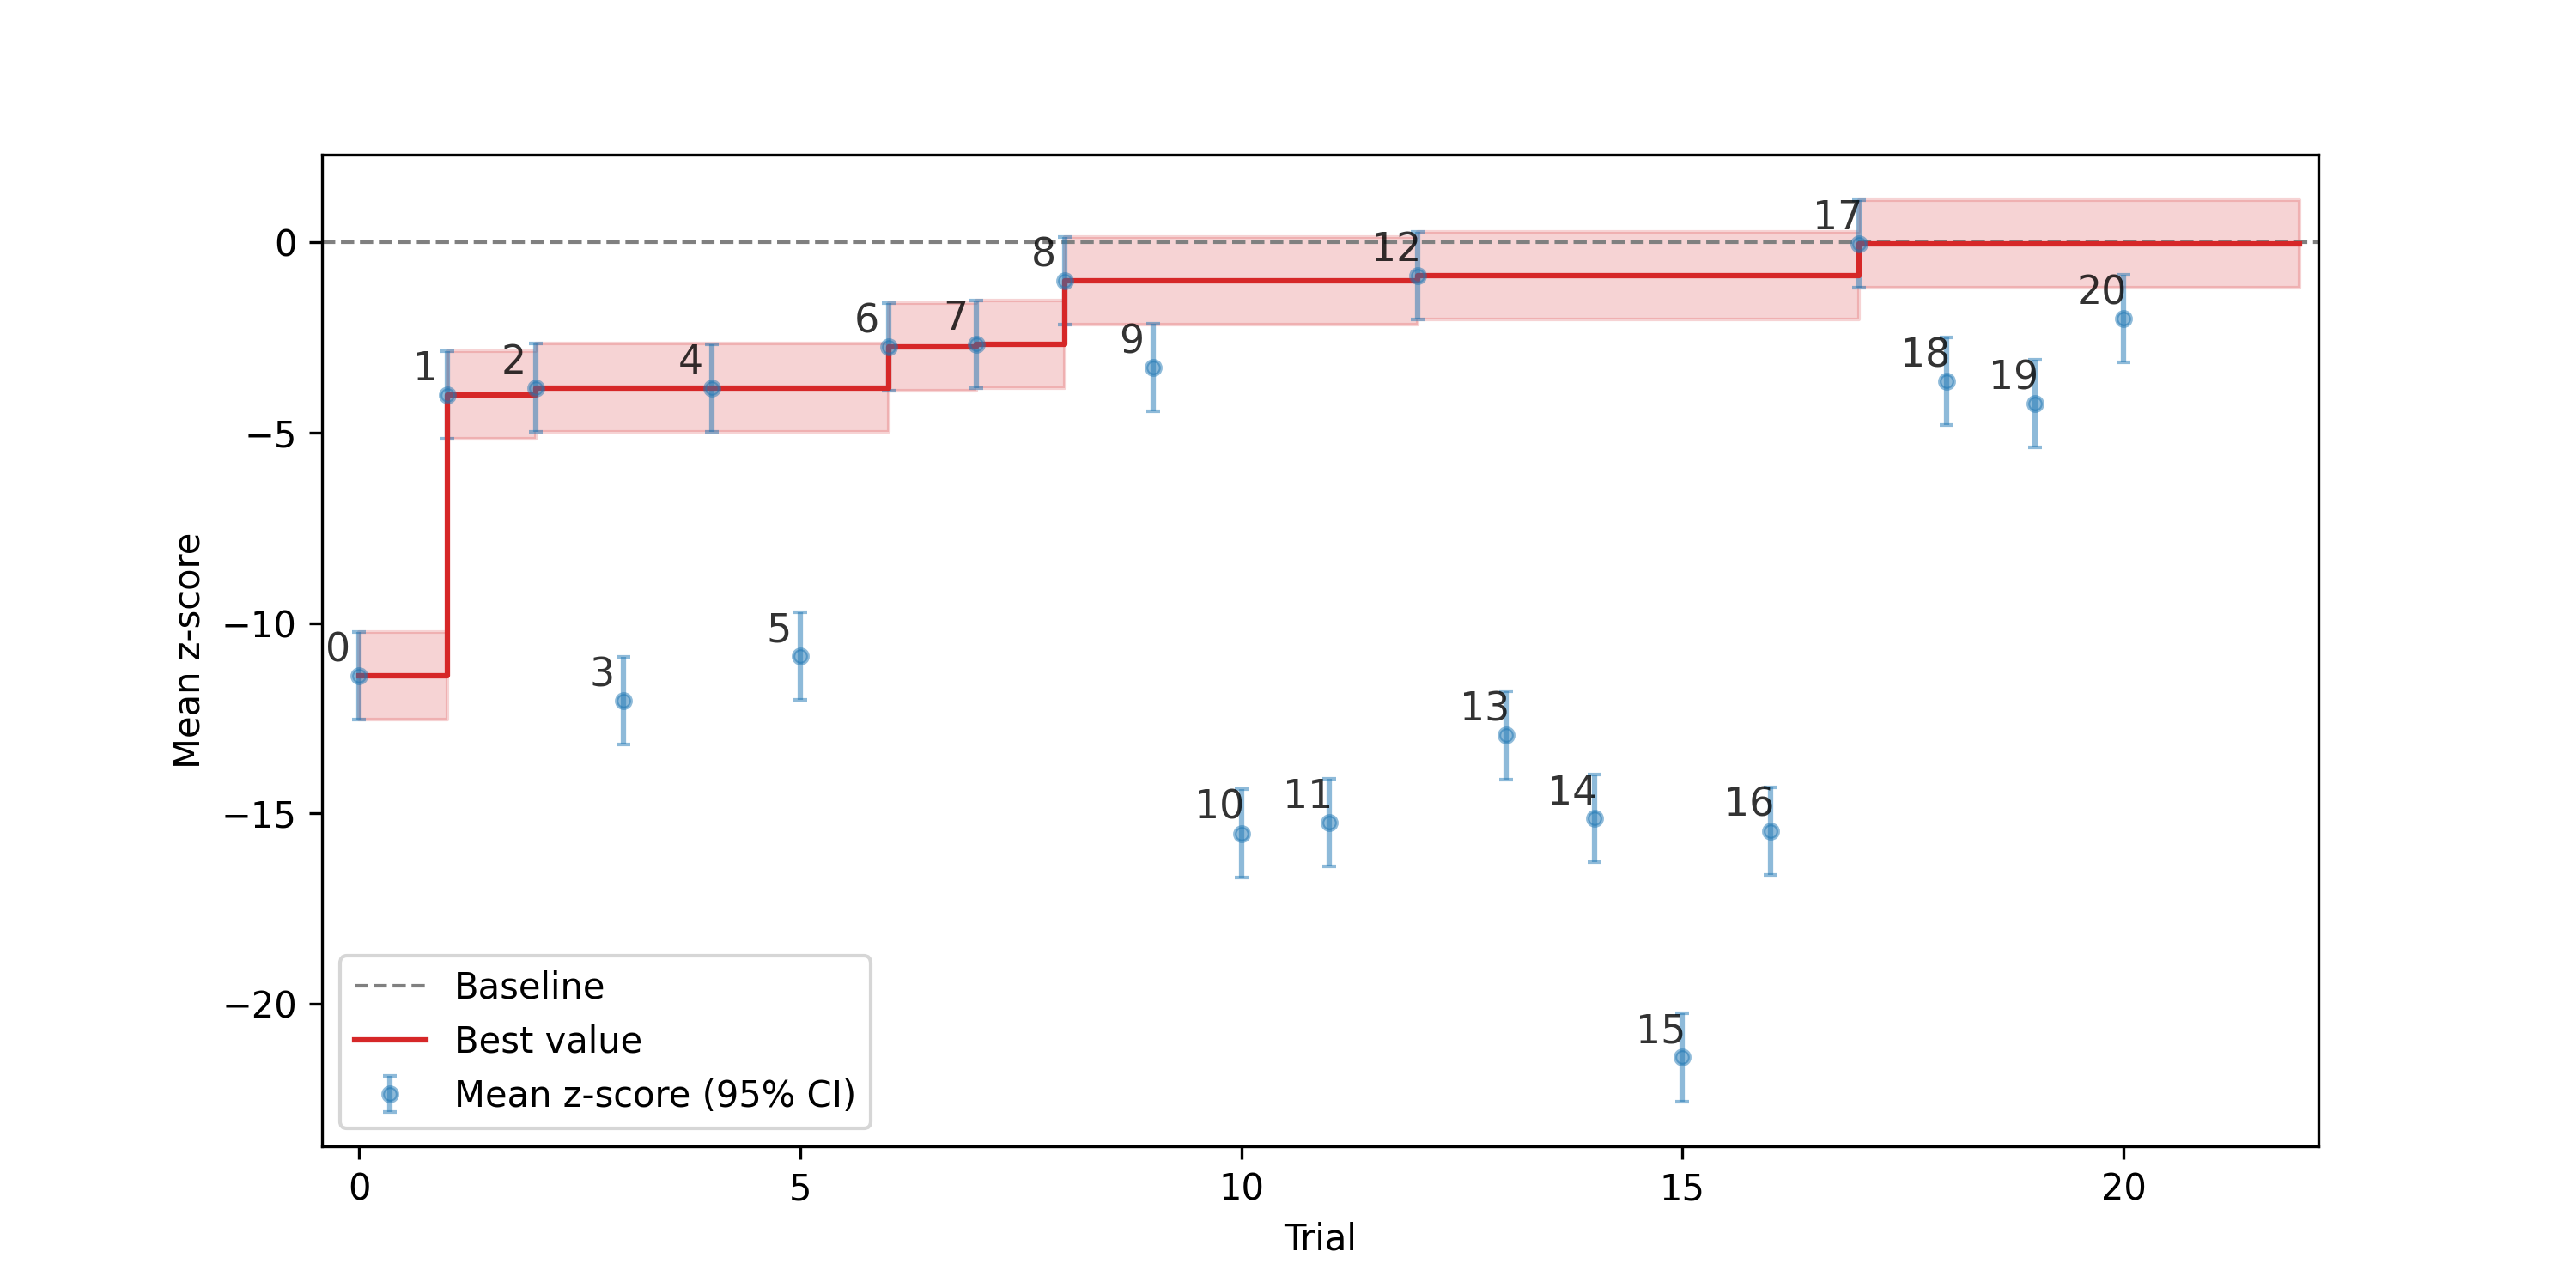
\includegraphics[width=\textwidth]{charts/trial_scores_confidence_interval.png}
	\caption{Optimization history showing the mean z-scores and their confidence interval for each trial}
\end{figure}

\begin{figure}[H]
	\centering
	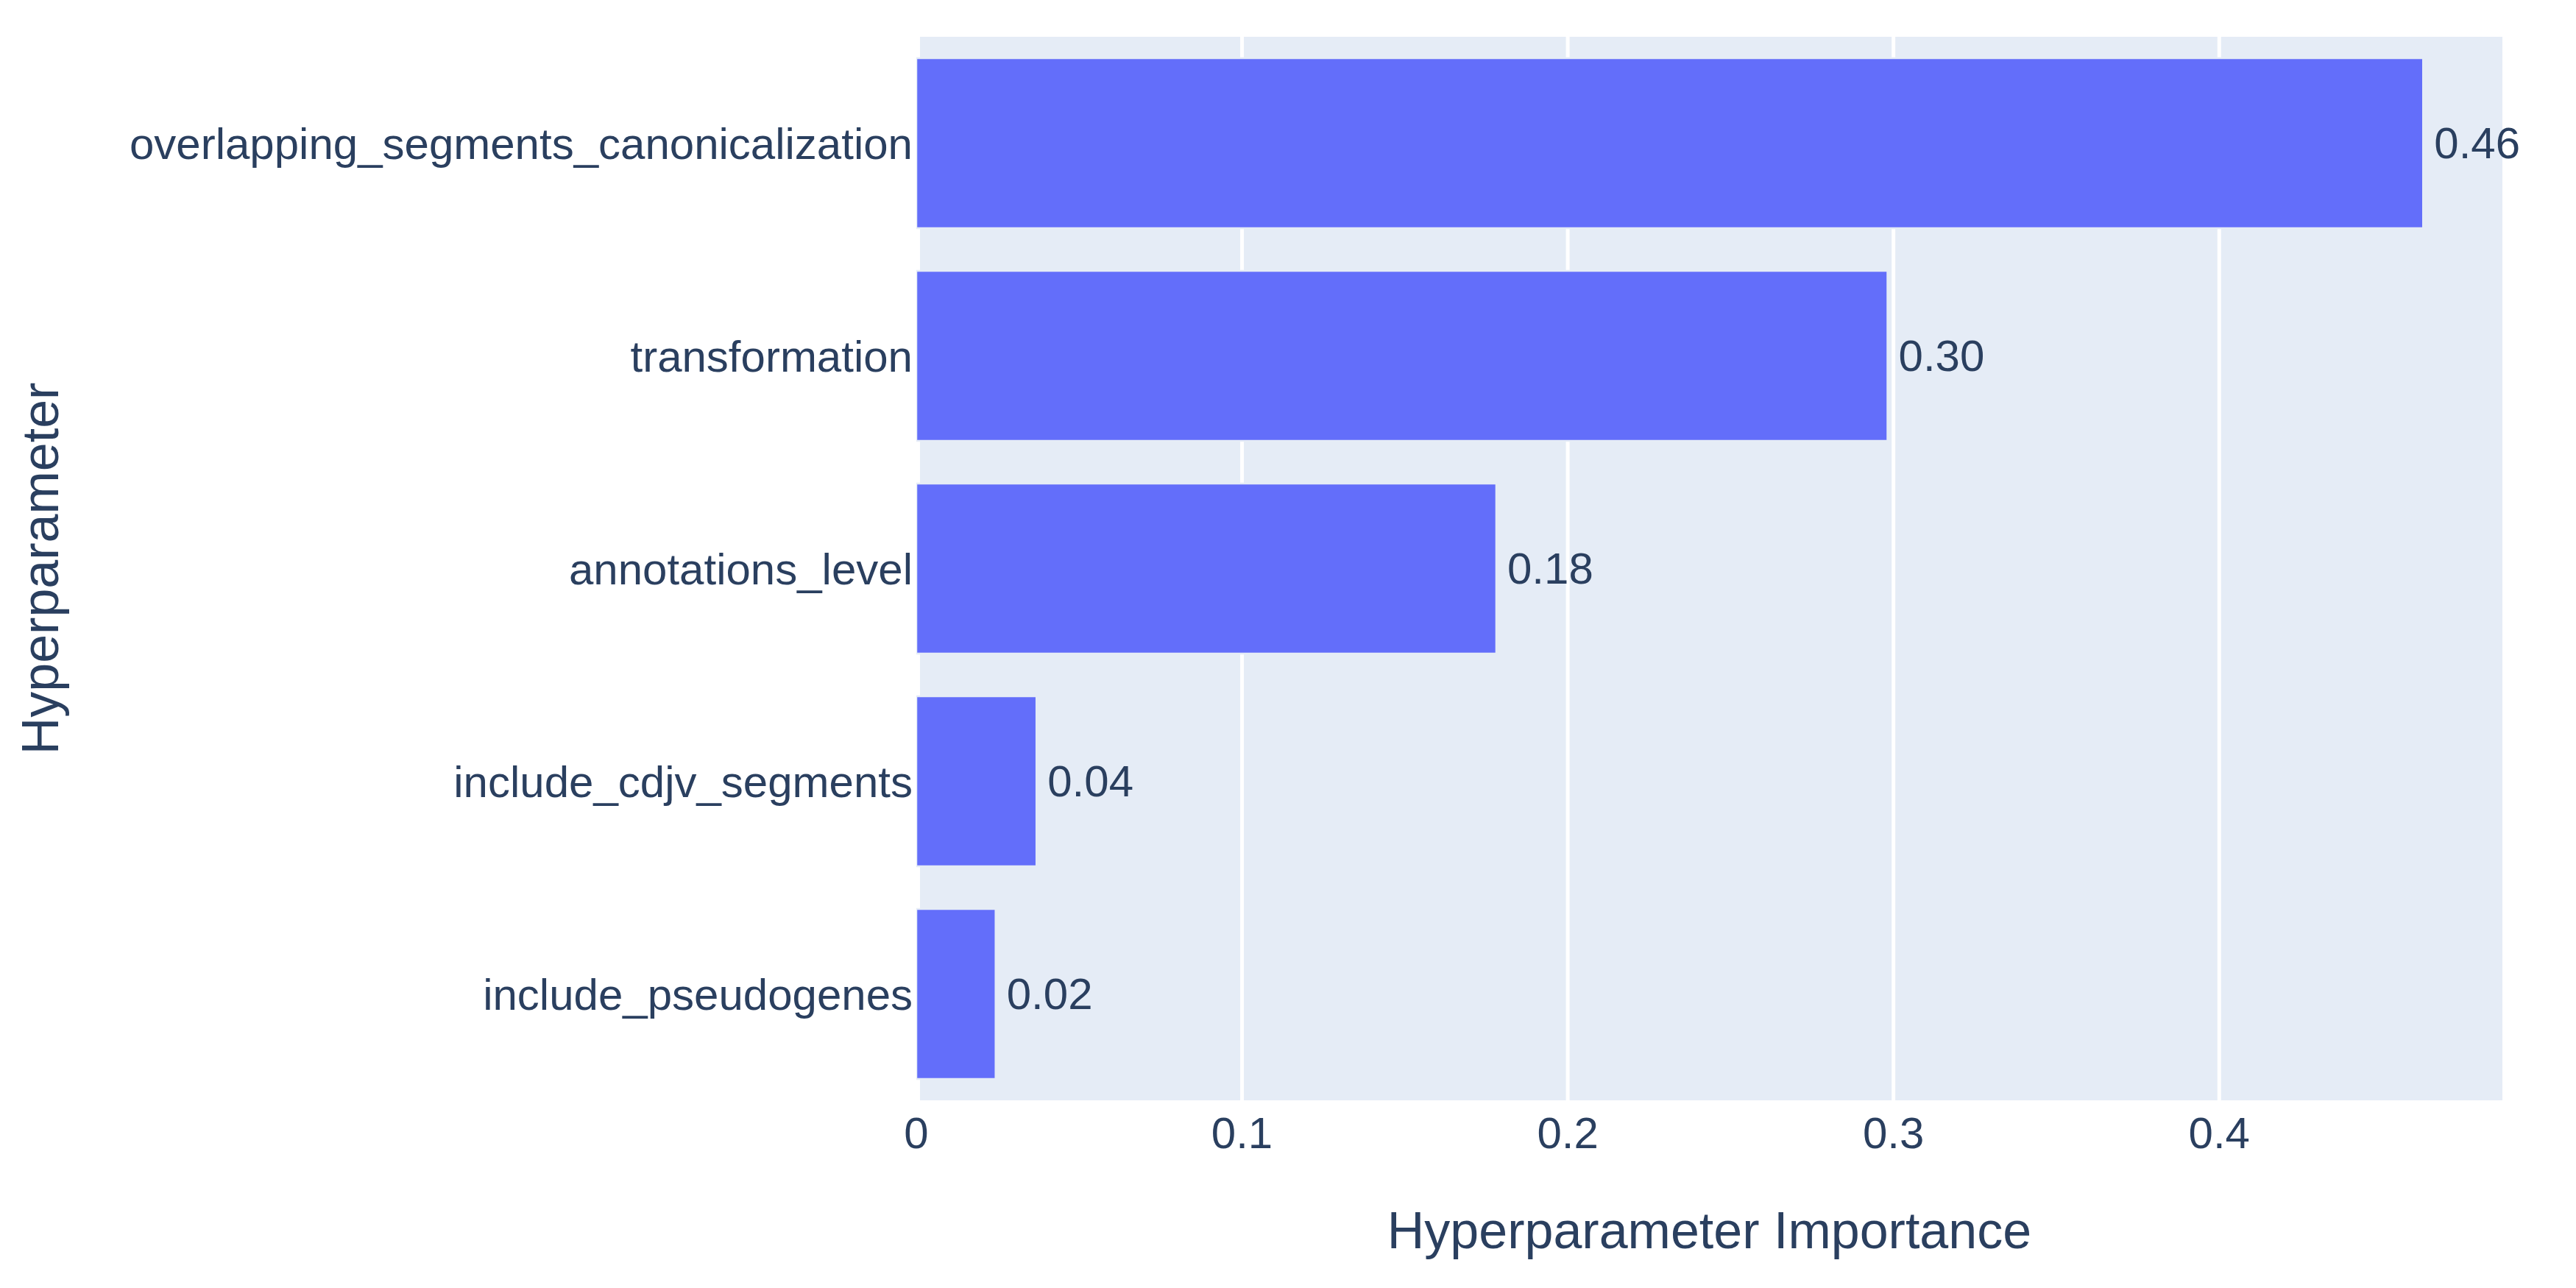
\includegraphics[width=0.7\textwidth]{charts/hpo_parameters_importance.png}
	\caption{Hyperparameter importance plot produced by Optuna}
\end{figure}

\section{Discussion}
\subsection{Interpreting the results}
As it can be seen, even though the leakage control model produces an improvement, it can't be discerned whether it comes from the model exploiting the transcriptional asymmetry, or some other reason (like the possible data leakage mentioned on section \ref{sec:methods_evaluation_canonicalizaiton_algorithms}). What is certain is that even if allowing the model to exploit that asymmetry is beneficial, implementing that exploitation through canonicalization doesn't seem to yield an improved performance.

It's noted that even though there could be a small improvement on the \texttt{demo\_human\_or\_worm} task from Genomic Benchmark, it can't be known (assuming there's a true improvement) if it comes from the exploitation of transcriptional asymmetry, or through simpler reasons, like the difference in length, frequency and number of genes in human vs C. elegans genomes \citep{eichingerGenomeSocialAmoeba2005}

\subsection{Future work}.
Regarding future work, one could:
\begin{itemize}
	\item Try to find another way to incorporate the transcriptional asymmetry into a model to assess whether this information can be exploited for better performance
	\item Modify the data used by the canonicalization method to evaluate it on the exploitation of the replicational asymmetries also mentioned by \citet{moeckelStrandAsymmetriesGenomic2023}
	\item Evaluate the canonicalization method on a different non-RC-equivariant architecture, like HyenaDNA\citep{nguyenHyenaDNALongRangeGenomic2023}
\end{itemize}

\subsection*{Reproducibility}
The code for the project can be found on \href{https://github.com/PipeVerri/Canonicalization}{Github}, with further guidance on how to reproduce the results there.

\subsection*{Acknowledgments}
My thanks go to E. Matias Castro for valuable guidance on the research process.

% --- Bibliografía ---
\bibliography{iclr2027_conference.bib}
\bibliographystyle{iclr2027_conference}

\appendix
\section{Appendix}

\subsection{Design of the canonicalization algorithm for overlapping transcripts}\label{sec:design-of-the-canonicalization-algorithm}
Regarding the approach to dealing with overlapping segments, 3 variables were proposed with which to formulate all the
hypotheses of the optimal algorithm: 

\begin{itemize}
	\item \emph{\texttt{overlap\_transformation\_behavior}}: Determines the different hypotheses for what happens when canonicalizing a segment \textbf{A} that overlaps with a segment \textbf{B}:
	\begin{itemize}
		\item \emph{Partial break}: Only the overlapping part between \textbf{A} and \textbf{B} of both segments breaks.
		\item \emph{Full break}: The entire segment \textbf{B} is broken when partially
		canonicalizing one of its parts.
		\item \emph{Both break}: Both \textbf{A} and \textbf{B} are entirely broken, since that overlapping part needed to be kept intact for both segments to be understood correctly by the model.
	\end{itemize}
	
	\begin{figure}[H]
		\centering
		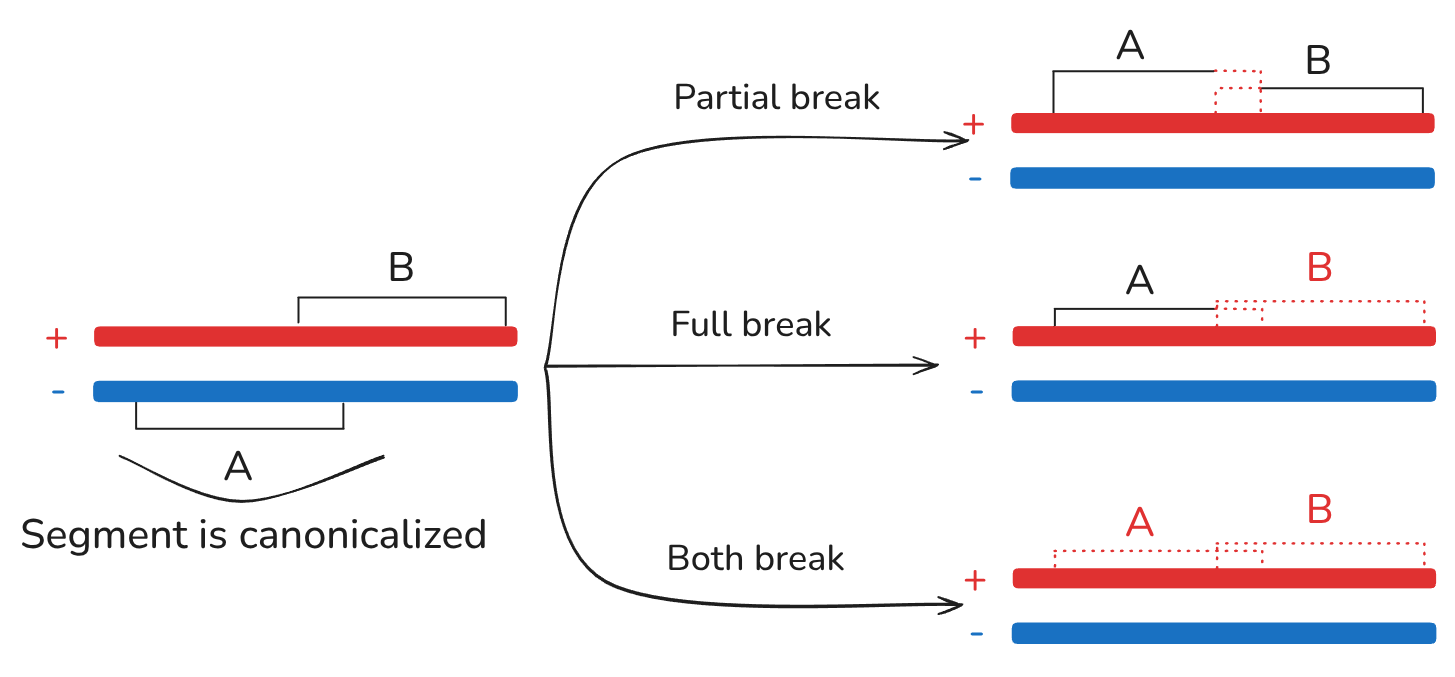
\includegraphics[width=0.7\textwidth]{overlap_break_behavior.png}
	\end{figure}
	
	\item \emph{\texttt{orient\_all\_segments}}: A binary variable indicating whether it
	is necessary for all segments to be in the canonical orientation, or
	whether to not canonicalize certain segments if the cost of ignoring
	them (the number of nucleotides) is lower than the cost of
	canonicalizing them (the number of nucleotides it destroys, which is
	calculated depending on \texttt{overlap\_transformation\_behavior}). The
	only case where it is not irrelevant is where
	\texttt{overlap\_transformation\_behavior = full\_break}; it is irrelevant in
	the rest of the cases. This is explained in more detail below.
	
	\item \emph{\texttt{keep\_segments\_order}}: In the case where
	\texttt{overlap\_transformation\_behavior = full\_break} and
	\texttt{orient\_all\_segments=True} there are 2 ways to canonicalize the
	segments, one that breaks the fewest nucleotides but destroys the
	original order of the segments, and another where that original order is
	kept but more nucleotides are destroyed. This variable decides which of
	the 2 ways to use. They are described in more detail below
\end{itemize}

Based on all the possible permutations of these variables, the following
canonicalization methods arise:
\begin{enumerate}
	\item If \texttt{overlap\_transformation\_behavior=partial\_break},
	\texttt{orient\_all\_segments} (and \texttt{keep\_segments\_order}) have no effect since the cost of ignoring a segment is always \(\geq\) the cost
	of canonicalizing it, since the length of the overlap is always less
	than or equal to the length of the segment, so all segments are
	oriented, regardless of whether there is an overlap or not
	\\
	\item If \texttt{overlap\_transformation\_behavior=full\_break}, there are 3
	possible canonicalization algorithms. They all rely on building a \emph{conflict window} first. When a negative segment that overlaps with a positive one is found, the entire conflict window is computed recursively, the set of the whole ``chain'' of overlapping segments.
	
	The reason conflict windows are used instead of simply looking at
	immediate overlaps, is that there are cases where only looking at
	immediate overlaps ends up in a bad decision. As shown in Figure~\ref{fig:conflict_window_example}, for example,
	if I decide whether to canonicalize \textbf{A} or not:
	\begin{enumerate}[label=\alph*]
		\item If I only check the immediate overlaps, then I do not canonicalize \textbf{A} since it is
		preferable to destroy it rather than \textbf{B} (because \textbf{B} is longer)
		
		\item If I check the entire conflict window, it is preferable for me to canonicalize the
		negative segments (100bp) and destroy \textbf{B} rather than ignore them.
	\end{enumerate}
	
	\begin{figure}[H]
		\centering
		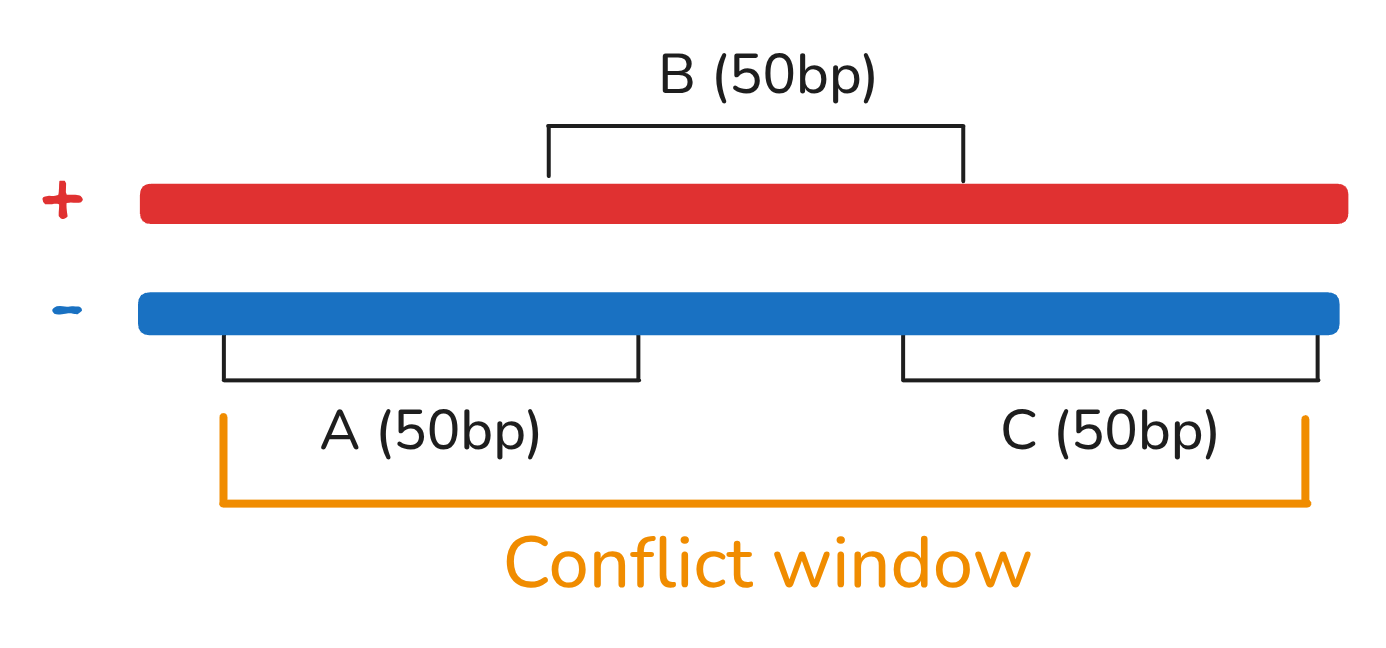
\includegraphics[width=0.5\textwidth]{conflict_window.png}
		\caption{Example showing the reason behind the usage of conflict windows}
		\label{fig:conflict_window_example}
	\end{figure}
	
	After the conflict window is built, the canonicalization algorithm branches in:
	\begin{enumerate}
		\item If \texttt{orient\_all\_segments=False}, then the cheapest option is chosen. Orient the negative segments at the cost of destroying the positive ones (the sum of the lengths of positive segments in the conflict window), or ignore the negative segments, at a cost equal to the sum of their lengths.
		
		\item If \texttt{orient\_all\_segments=True}, then there are 2 ways to deal with the overlapping segments:
		
		\begin{enumerate}
			\item If one wishes to keep the exact order of the segments as they were (\texttt{keep\_segments\_order=True}), then, across the whole genome, one can either canonicalize the segments from the - to the + strand in all of the conflict windows, or canonicalize the segments from the + to the - strand, and then take the RC of the entire genome to bring them all to the + strand.
			
			\medskip
			Although the original order of the segments is not maintained when applying the second option, relative order of ``which one follows which'' is still maintained. An example of this canonicalization method can be seen on Figure~\ref{fig:canon_ordered_segments}
			
			\begin{figure}[H]
				\centering
				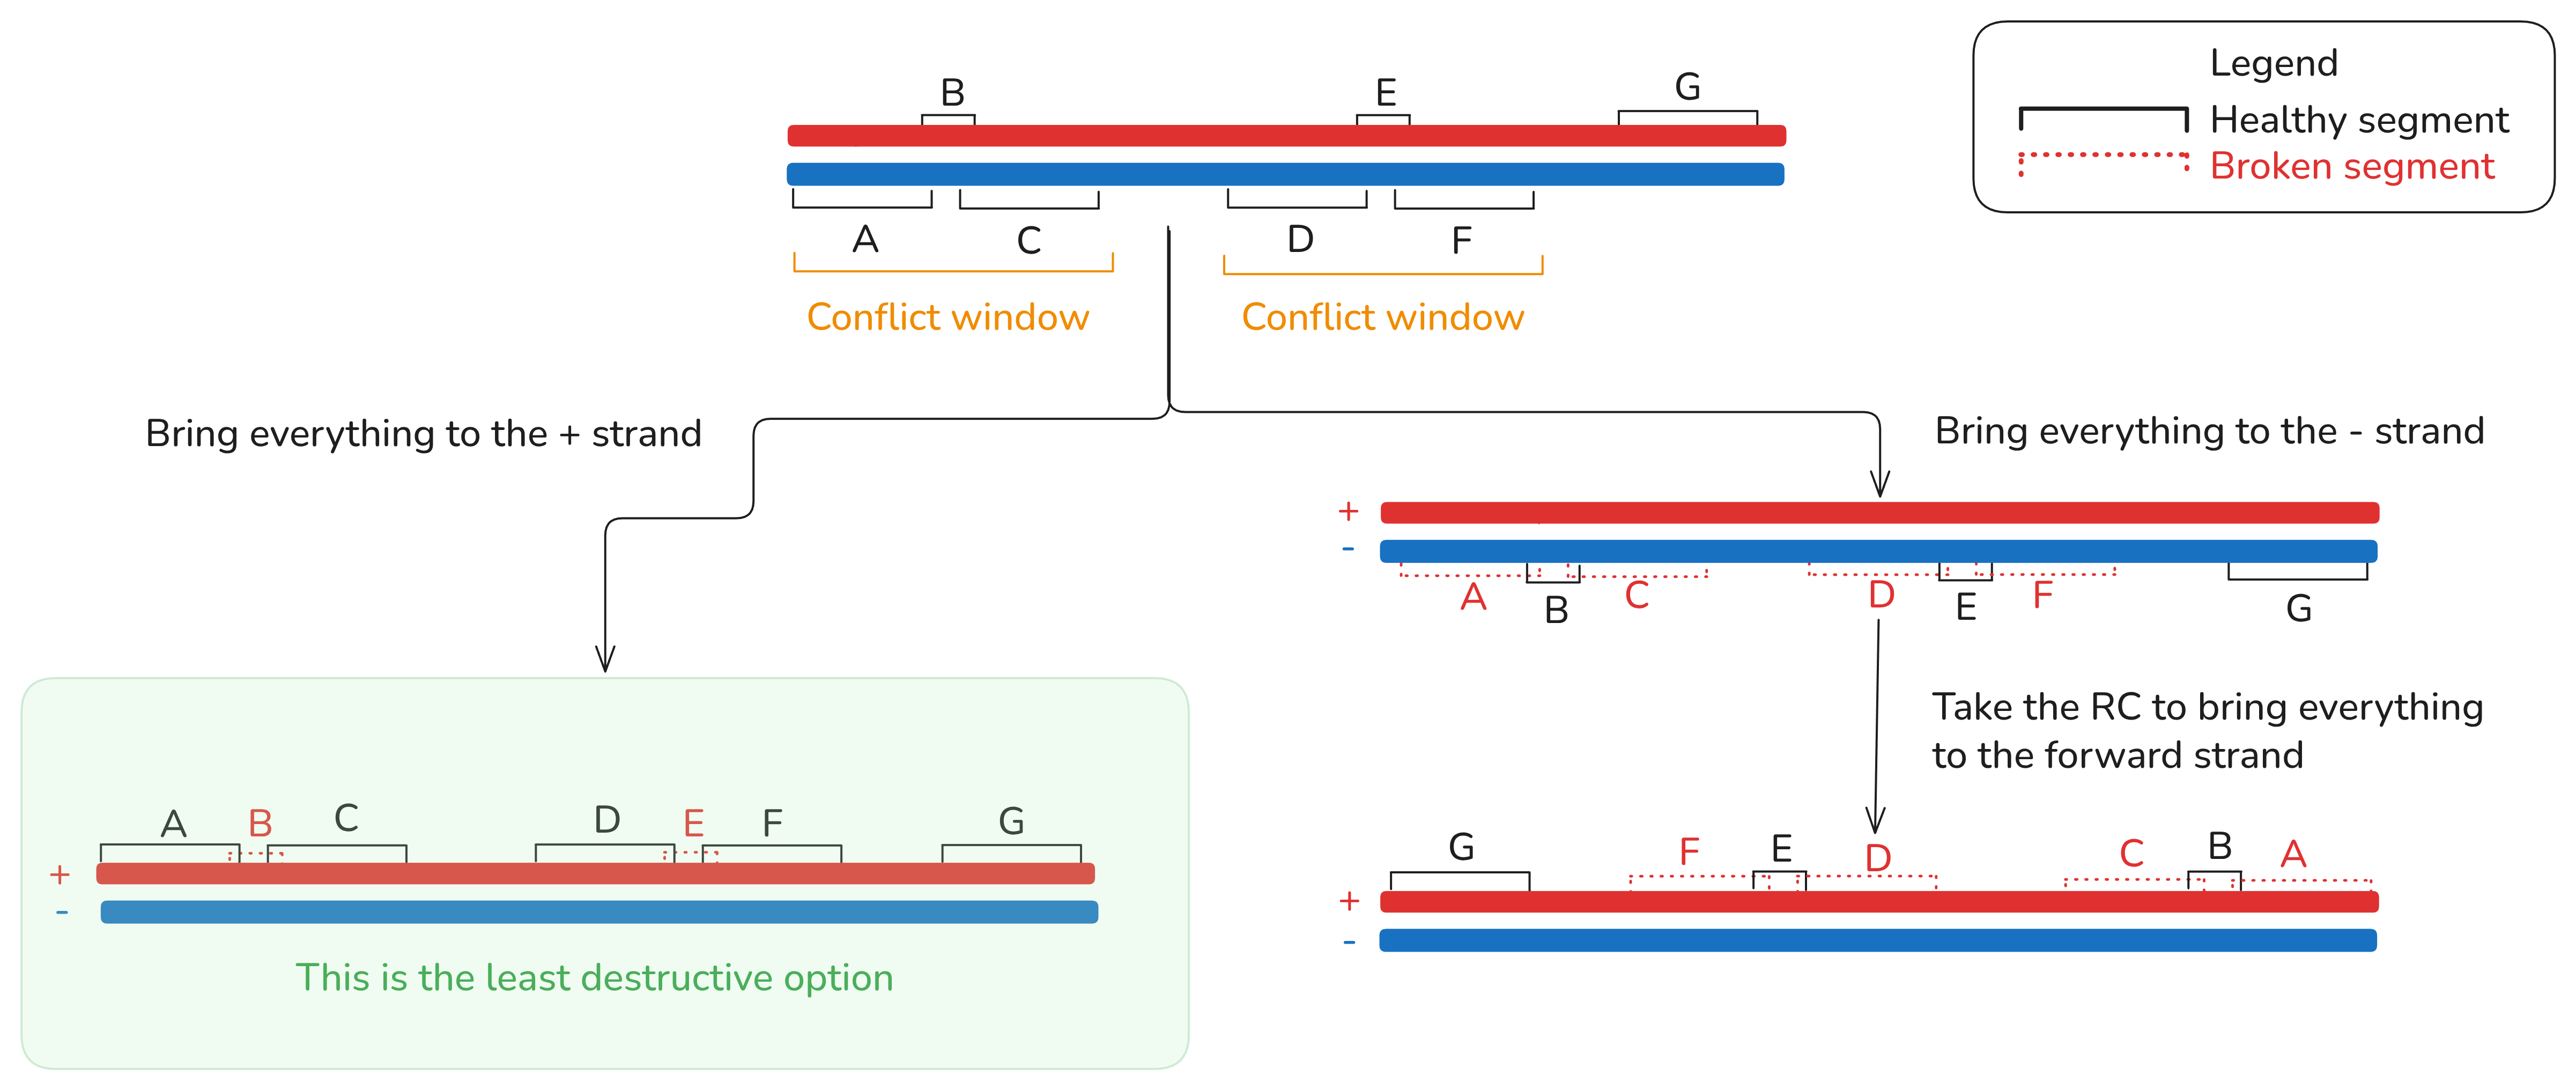
\includegraphics[width=\textwidth]{ordered_segments_canonicalization.png}
				\caption{}
				\captionsetup{labelsep=none}
				\label{fig:canon_ordered_segments}
			\end{figure}
			
			
			\item If the canonicalization with the lowest total cost is desired, regardless of the order of the segments, a procedure similar to the previous one is applied but with scope at the overlap window level instead of the genomic level. The reason the order is lost is that some overlap windows are reversed and others are not, causing the order to be lost at the genomic level. An example of this method can be seen below on Figure~\ref{fig:keep_order_false_example}
			
			\begin{figure}[H]
				\centering
				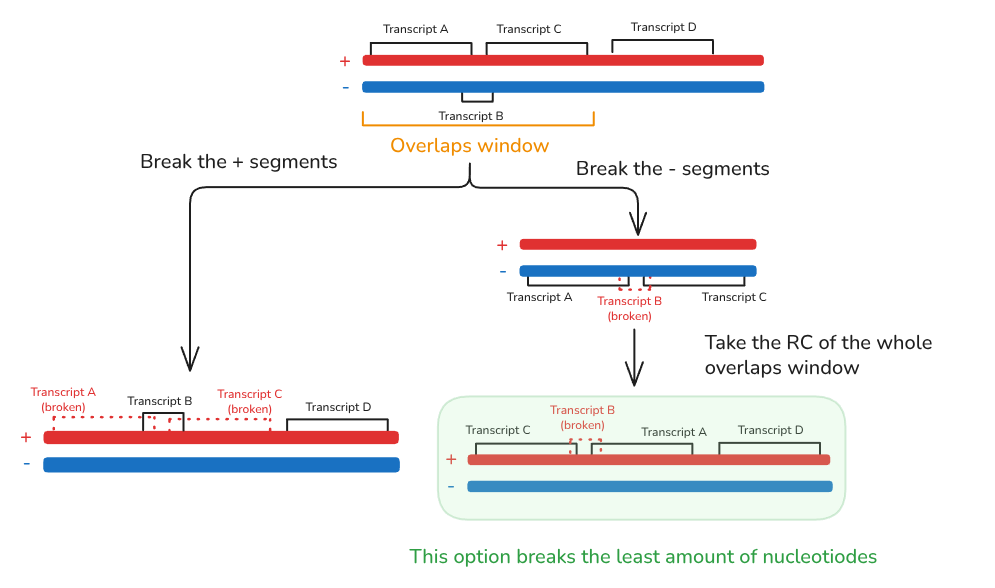
\includegraphics[width=\textwidth]{keep_order_false_example.png}
				\caption{}
				\captionsetup{labelsep=none}
				\label{fig:keep_order_false_example}
			\end{figure}
		\end{enumerate}
	\end{enumerate}
	
	\item If \texttt{overlap\_transformation\_behavior=both\_break}, there are two possible canonicalization algorithms. Both algorithms consist of canonicalizing the segments that don't overlap with any segments on the opposite strand, and for the ones that do, instead of canonicalizing them --- which would always cost more, because the cost of canonicalizing them (length(\textbf{A}) + length(\textbf{B})) is always higher than the cost of ignoring them (length(\textbf{A})) --- it's chosen whether to keep the positive strand of the segments or the negative one, depending on which strand has the most amount of coding nucleotides.
	\begin{enumerate}
		\item If \texttt{keep\_segments\_order=True} the algorithm chooses whether to canonicalize the non-overlapping negative segments, or to canonicalize the non-overlapping positive segments and then take the RC of the whole sequence
		\item If \texttt{keep\_segments\_order=False}, the algorithm canonicalizes all the non-overlapping negative segments, and then, for each conflict window, it decides whether to leave it as-is or to canonicalize it.
	\end{enumerate}
	
	This algorithm is similar to the one used when \texttt{overlap\_transformation\_behavior=full\_break} and \texttt{orient\_all\_segments=False}, the only difference is in that case, all the segments(including the ones that have overlaps) are canonicalized.
\end{enumerate}

The advantages and disadvantages of the possible configurations of
\texttt{keep\_segments\_order} can be seen on Figure~\ref{fig:full_break_examples}.
\begin{itemize}
	\item In the case where \texttt{keep\_segments\_order=True}, the canonicalization is done that way because destroying the B, D and F segments (110bp) is cheaper than destroying the A, C and E segments (210bp)
	\item In the case where \texttt{keep\_segments\_order=False} each overlap window is processed individually, and even though the result destroys the least amount of nucleotides, the order is lost (as seen in the second conflict window)
\end{itemize}

\begin{figure}[H]
	\centering
	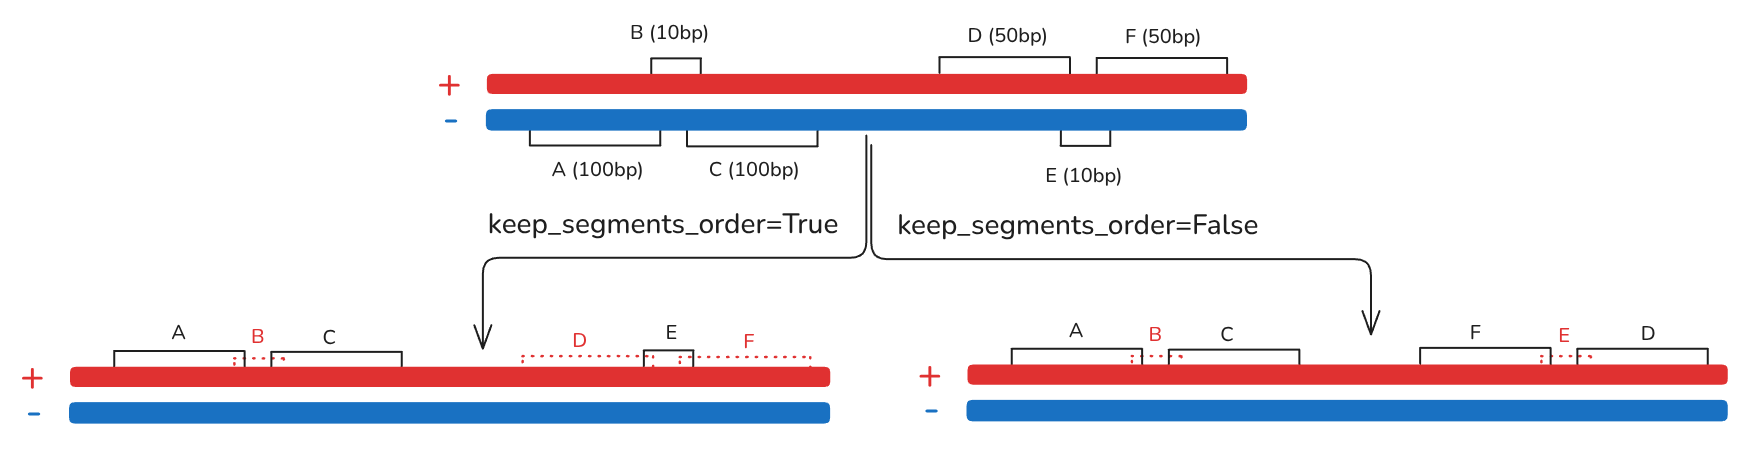
\includegraphics[width=\textwidth]{canonicalization_algorithms_example.png}
	\caption{}
	\captionsetup{labelsep=none}
	\label{fig:full_break_examples}
\end{figure}

\subsection{Model parameters}

It's worth noting that \texttt{d\_inner} determines the dimension of the middle layers of the MLP that comes before the downstream head, as seen on the figure below

\begin{figure}[H]
	\centering
	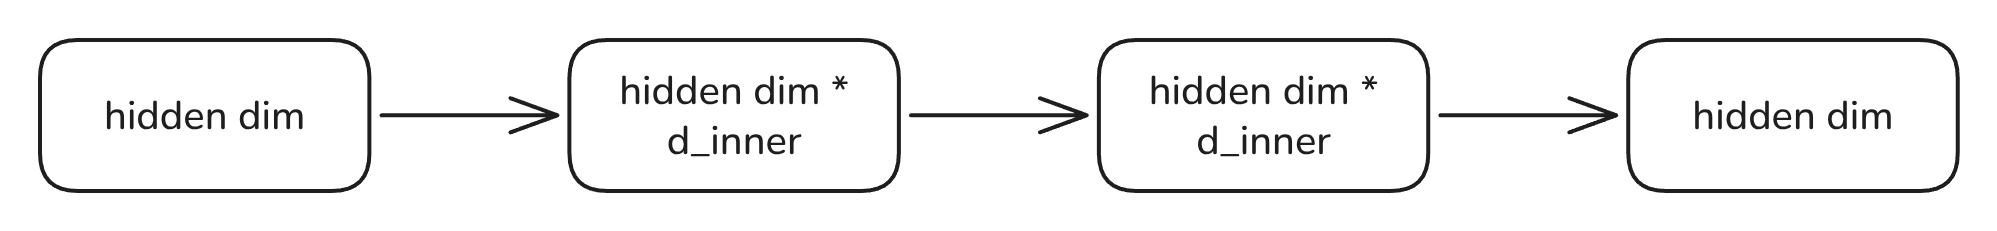
\includegraphics[width=\textwidth]{mlp_final_layer.png}
\end{figure}

\subsubsection{Pretraining}
The same configuration as the original
ConvNova paper was used, which used a configuration similar to HyenaDNA.

{\def\LTcaptype{none} % do not increment counter
	\begin{longtable}[]{@{}ll@{}}
		\toprule\noalign{}
		Hyperparameter & Value \\
		\midrule\noalign{}
		\endhead
		\bottomrule\noalign{}
		\endlastfoot
		Learning Rate & \(\beta_1=0.9, \beta_2=0.999\) \\
		Batch Size & 256 \\
		Weight Decay & 0.1 \\
		Dropout & 0.0 \\
		Optimizer & AdamW \\
		Optimizer Momentum & \(\beta_1=0.9, \beta_2=0.999\) \\
		Learning Rate Scheduler & Cosine Decay \\
		\midrule
		Epochs & 400 \\
		Dilation rate & 4 \\
		Precision & fp32 \\
		Kernel size & 9 \\
	\end{longtable}
}

Different sequence lengths were used for each model:

{\def\LTcaptype{none} % do not increment counter
	\begin{longtable}[]{@{}lllll@{}}
		\toprule\noalign{}
		Parameters & 378k & 1.7M & 6.8M & 7.4M \\
		\midrule\noalign{}
		\endhead
		\bottomrule\noalign{}
		\endlastfoot
		Sequence length & 1k & 1k & 1k & 2k \\
	\end{longtable}
}

\subsubsection{Downstream tasks}\label{sec:appendix_downstream_tasks}

The same configuration as for pretraining was used but with the
following changes. The configuration is similar to the one used in ConvNova, with a slight difference in the sequence length for Genomic Benchmark. While they trained ConvNova on Genomic Benchmark with a sequence length of 1k (to have a direct comparison against transformer-based models), some tasks on Genomic Benchmark have an actual higher sequence length (one of the tasks, for example, has a sequence length of 5k), and it was decided to use those true sequence lengths to have a more accurate representation of the canonicalization algorithm's performance.

Note that for the Genomic Benchmark, even though the original ConvNova paper reports a 386k parameter model for this task, the configurations provided in the paper and its GitHub repo don't match this parameter count. The authors were contacted with no response, so the configuration that comes closest to 386k parameters, a 378k one, was chosen.

\begin{table}[ht]
	\centering
	% Nota que se usa tabularx, se define el ancho {\textwidth} y se agregó \\ al final
	\begin{tabularx}{\textwidth}{X X c c c c}
		\toprule
		Task & Sequence Length & Hidden dim & Num GCBs & Size & \texttt{d\_inner} \\
		\midrule
		NT Benchmark & 1k & 128 & 5 & 1.7M & 2 \\
		Genomic Benchmark & Depends on the task, shown below & 64t & 5 & 378k & 4 \\
		BEND Benchmark & 512 for CpG methylation, 16k for gene finding & 196 & 10 & 7.4M & 2 \\
		Chromatin Profile Prediction & 1k & 256 & 5 & 6.8M & 2 \\
		\bottomrule
	\end{tabularx}
\end{table}

\begin{table}[htbp]
	\centering
	\caption{Sequence lengths for Genomic Benchmark}
	\begin{tabular}{lc}
		\toprule
		Task & Sequence length \\
		\midrule
		dummy\_mouse\_enhancers\_ensembl & 5000 \\
		demo\_coding\_vs\_intergenomic\_seqs & 200 \\
		demo\_human\_or\_worm & 200 \\
		human\_enhancers\_cohn & 500 \\
		human\_enhancers\_ensembl & 573 \\
		human\_ensembl\_regulatory & 802 \\
		human\_nontata\_promoters & 251 \\
		human\_ocr\_ensembl & 600 \\
		drosophila\_enhancers\_stark & 3250 \\
		\bottomrule
	\end{tabular}
\end{table}

\subsubsection{Hyperparameter search}\label{hyperparameter-search}

For the hyperparameter search, the model was pretrained and fine-tuned
on all tasks with the same pretraining and downstream tasks
configuration, but with the following differences across all of them.

It should be noted that a single pretrained model per trial was used for
the rest of the downstream tasks. The difference in precision was to speed up the hyperparameter search, \emph{and the number of pretraining epochs was also changed from 400 to 200.}

{\def\LTcaptype{none} % do not increment counter
	\begin{longtable}[]{@{}lllllll@{}}
		\toprule\noalign{}
		Hidden dim & Num GCBs & Kernel size & d\_inner & Size & Precision & Random seed \\
		\midrule\noalign{}
		\endhead
		\bottomrule\noalign{}
		\endlastfoot
		64 & 5 & 5 & 2 & 262k & bf16 & 2222 \\
	\end{longtable}
}

\subsection{Classification of tasks into RC-invariant, RC-equivariant, or omitted}
\label{sec:downstream-task-canon-classification}

Many benchmark tasks can generally be classified into tasks of histone
marks, enhancers, promoters, and splicing. These task classes were
treated as specified in the table below.

It is worth mentioning that tasks where the canonicalization was omitted were still evaluated because it was hypothesized that the canonicalized pretraining may change the performance of the model on those tasks.

\begin{xltabular}{\textwidth}{p{3cm} p{1.8cm} X}
	\caption{\textbf{Classification and rationale for genomic tasks}} 
	\label{tab:genomic_tasks_classification} \\
	\toprule
	Task & Class & Reason \\
	\midrule
	\endfirsthead
	
	\multicolumn{3}{c}%
	{{\tablename\ \thetable{} -- Continuation of the previous page}} \\
	\toprule
	Task & Class & Reason \\
	\midrule
	\endhead
	
	\bottomrule
	\endfoot
	
	Histone marks tasks and OCR (open chromatin region) tasks & RC-invariant & Histones interact with double-stranded DNA, so their marks are invariant to the RC of the sequence. The same applies to OCR tasks. \\
	\midrule
	Enhancer tasks & RC-invariant & Most enhancers are functionally bidirectional\citep{arnoldGenomeWideQuantitativeEnhancer2013}, and in the majority of cases, both enhancer strands get transcribed into eRNA\citep{arnoldDiversityEmergingRoles2020}. Even so, it should be noted that there are special cases where enhancers are orientation-dependent, like in super-enhancers \citep{kassoufAglobinSuperenhancerActs2025}. \\
	\midrule
	Promoter tasks & Omitted & Promoters are inherently directional, since they only function on one of the strands --- otherwise, both strands would be transcribed. \par\medskip There is no way to know without experimental data whether the RC of a promoter is a promoter or not, or whether the RC of a non-promoter sequence produces a promoter. That is why they were omitted. \\
	\midrule
	Splicing tasks & Omitted & Applying the canonicalization to sequences that contain acceptor or donor sites should have no effect because the sequences passed are already on the positive coding strand. For the sequences without acceptor or donor sites, applying the canonicalization algorithm could invert the sequence's label if it falls on the template strand of a coding region, and I can't update the labels because I can't be certain of a sequence label without experimental data  \\
	
\end{xltabular}	

For the particular cases, the way each of them is handled is detailed below:

\subsubsection{Nucleotide Transformer Benchmark}
There are no particular tasks that don't fit within the classes mentioned above.

\subsubsection{Genomic Benchmark}
The only tasks that don't fit within the classes mentioned above are:
\begin{table}[htbp]
	\centering
	\caption{Classification and rationale for genomic tasks}
	
	\begin{tabularx}{\linewidth}{p{3cm} p{3cm} X}
		
		\toprule
		
		Task & Class & Reason \\
		
		\midrule
		
		\seqsplit{demo\_human\_or\_worm} & RC-invariant & The RC of human DNA is still human DNA; the same applies to any other species. \\
		
		\midrule
		
		\seqsplit{demo\_coding\_vs\_intergenomic\_seqs} & RC-invariant & Taking the RC of a sequence positioned on a transcribed feature does not move it outside that feature; it only changes its orientation. The same applies to non-transcribed sequences. \\
		
		\midrule
		
		\seqsplit{human\_ensembl\_regulatory} & RC-invariant for enhancers and OCR; promoter samples are omitted & The task consists of classifying a DNA sequence among enhancers, promoters, and OCR. What each strand is is identified using the labels, and promoters are omitted. \\
		
		\bottomrule
		
	\end{tabularx}
\end{table} 

\subsubsection{BEND Benchmark}

\begin{table}[H]
	\centering
	\caption{Classification and rationale for BEND Benchmark tasks}
	\label{tab:bend_benchmark}
	
	\begin{tabularx}{\linewidth}{p{3cm} p{3cm} X}
		\toprule
		Task & Class & Reason \\
		\midrule
		
		Gene finding & RC-equivariant & The task consists of classifying each nucleotide as \{exon forward, donor forward, intron forward, acceptor forward, exon reverse, ..., non-coding\}. Taking the RC of a coding nucleotide changes its orientation and changes its position. \\
		
		\midrule
		
		CpG Methylation & RC-invariant & The reverse complement of CG is CG, and they are both methylated on both strands \cite{birdUseRestrictionEnzymes1978}. \\
		
		\bottomrule
	\end{tabularx}
\end{table}

\subsubsection{Chromatin Profile Prediction}

Most transcription factors (TFs) are functionally invariant to the reverse complement\citep{coonsDecodingInversionSymmetry2019}, so the task
is treated as RC-invariant. 

\end{document}
